\documentclass[11pt]{amsart}
\usepackage{float}
\usepackage{amsfonts, amstext, amsmath, amsthm, amscd, amssymb, upgreek}
\usepackage{bbm}
\usepackage{graphicx, color,  subfigure, wrapfig, overpic}
%\usepackage[all,cmtip]{xy} 
\usepackage{tikz}
%\usepackage{mystyle}

\newcommand{\thmref}[1]{Theorem \ref{#1}}
\newcommand{\prpref}[1]{Proposition \ref{#1}}
\newcommand{\lemref}[1]{Lemma \ref{#1}}
\newcommand{\figref}[1]{Figure \ref{#1}}
\newcommand{\comment}[1]{}


\textwidth 6.07in 
\textheight 8.6in 
\oddsidemargin 0.18in
\evensidemargin 0.18in
% \topmargin -0.07in
 
%%  If the following line is uncommented, we see the labels of theorems, figures, etc. in the margins.
% \usepackage[notref,notcite]{showkeys}
\setlength{\marginparwidth}{0.8in}
\let\oldmarginpar\marginpar
\renewcommand\marginpar[1]{\oldmarginpar[\raggedleft\footnotesize #1]%
{\raggedright\footnotesize #1}}

%This command stops the Math Review numbers appearing in the references! 
\AtBeginDocument{
   \def\MR#1{}
}
\newcommand{\Sp}{{\rm{S}}}
\newcommand{\C}{\mathbb{C}}
\newcommand{\R}{\mathbb{R}}
\newcommand{\Q}{\mathbb{Q}}
\newcommand{\Z}{\mathbb{Z}}
\newcommand{\N}{\mathbb{N}}
\newcommand{\CC}{\mathbb{C}}
\newcommand{\RR}{\mathbb{R}}
\newcommand{\HH}{\mathbb{H}}
\newcommand{\ZZ}{\mathbb{Z}}
\newcommand{\bfloor}[1]{\left\lfloor #1\right\rfloor}
\renewcommand{\P}{\mathcal P}
\newcommand{\A}{\mathcal A}
\newcommand{\W}{\mathcal W}
\newcommand{\vol}{{\rm vol}}
\newcommand{\cut}{{\backslash \backslash}}
\newcommand{\bdy}{\partial}
\newcommand{\voct}{{v_{\rm oct}}}
\newcommand{\vtet}{{v_{\rm tet}}}
\renewcommand{\L}{\mathcal L}
\newcommand{\cp}{\mathcal{C}}
\newcommand{\toF}{{\overset{F}{\longrightarrow}}}
\newcommand{\K}{\upkappa}

\def\co{\colon\thinspace}


\newcommand{\torus}{{\mathbb{T}^2}}
\newcommand{\sT}{{\mathcal{T}}}

\newcommand{\RRR}{{\underline{\mathfrak{R}}}}
\newcommand{\QQQ}{{\underline{\mathfrak{Q}}}}
\newcommand{\CCC}{{\underline{\mathfrak{C}}}}
\newcommand{\PPP}{{\underline{\mathbf{\Phi}}}}
\newcommand{\TTT}{{\underline{\mathbf{\Theta}}}}
\newcommand{\LLL}{{\underline{\mathfrak{L}}}}

\newcommand{\cev}[1]{\overset{\leftarrow}{#1}}

\newcommand{\del}{\partial}
\newcommand{\ddd}[1]{{\frac{\del}{\del #1}}}
\newcommand{\vphi}{\varphi}
\newcommand{\veps}{\varepsilon}
\newcommand{\llong}{{\text{long}}}
\newcommand{\Span}{{\text{span}}}
\newcommand{\Pol}{{\text{Pol}}}
\newcommand{\toruscomp}[1]{{\torus \times I - #1}}

\theoremstyle{plain}
\newtheorem{theorem}{Theorem}[section]
\newtheorem{corollary}[theorem]{Corollary}
\newtheorem{lemma}[theorem]{Lemma}
\newtheorem{prop}[theorem]{Proposition}
\newtheorem{claim}[theorem]{Claim}
\newtheorem{conjecture}[theorem]{Conjecture}
\newtheorem{example}[theorem]{Example}

\newtheorem*{namedtheorem}{\theoremname}
\newcommand{\theoremname}{testing}
\newenvironment{named}[1]{\renewcommand{\theoremname}{#1}\begin{namedtheorem}}{\end{namedtheorem}}
\theoremstyle{definition}
\newtheorem{define}[theorem]{Definition}
\newtheorem{definition}[theorem]{Definition}
\newtheorem{question}[theorem]{Question}
\newtheorem{remark}[theorem]{Remark}

\title [Augmented Links in the Thickened Torus] {Augmented Links in the Thickened Torus}


\author[Alice Kwon and Ying Hong Tham]{Alice Kwon and Ying Hong Tham}


\begin{document}
\maketitle

\begin{abstract}
  abstract goes here...
\end{abstract}

\section{Introduction}

Given a twist reduced diagram of a link $L$, {\it augmentation} is a process in which an unknotted circle component is added to one or more twist regions (a single crossing or a string of bigons) of $L$. Due to the added circle component we can remove full twists at the twist region of $L$. If the twist region has an odd number of crossings then all but one crossing is removed, whereas if the twist region has an even number of crossings then all are removed. The newly obtained link diagram is called an {\it augmented link diagram}. See Figure \ref{fig:Augmentations}.

Adams showed in \cite{CA} that given a hyperbolic alternating link $K$ in $\Sp^3$ the link $L$ obtained by augmentation $K$ is hyperbolic. In this paper we investigate if this statement holds for links in the thickened torus i.e. if $L$ is a link obtained from augmenting a hyperbolic alternating link $K$ in the thickened torus. In this chapter we find many families of hyperbolic links in the thickened torus which remain hyperbolic after augmentation. 
 \begin{figure}
 \centering  
 \begin{tabular}{cc}
 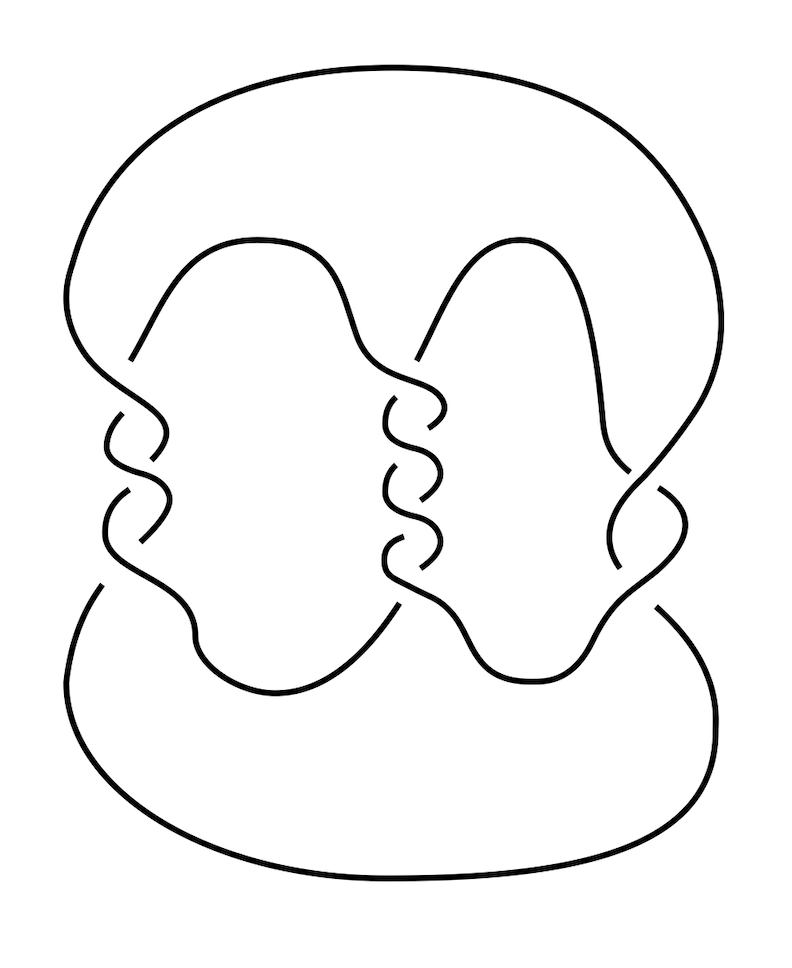
\includegraphics [height=4cm]{augmentation1}&
  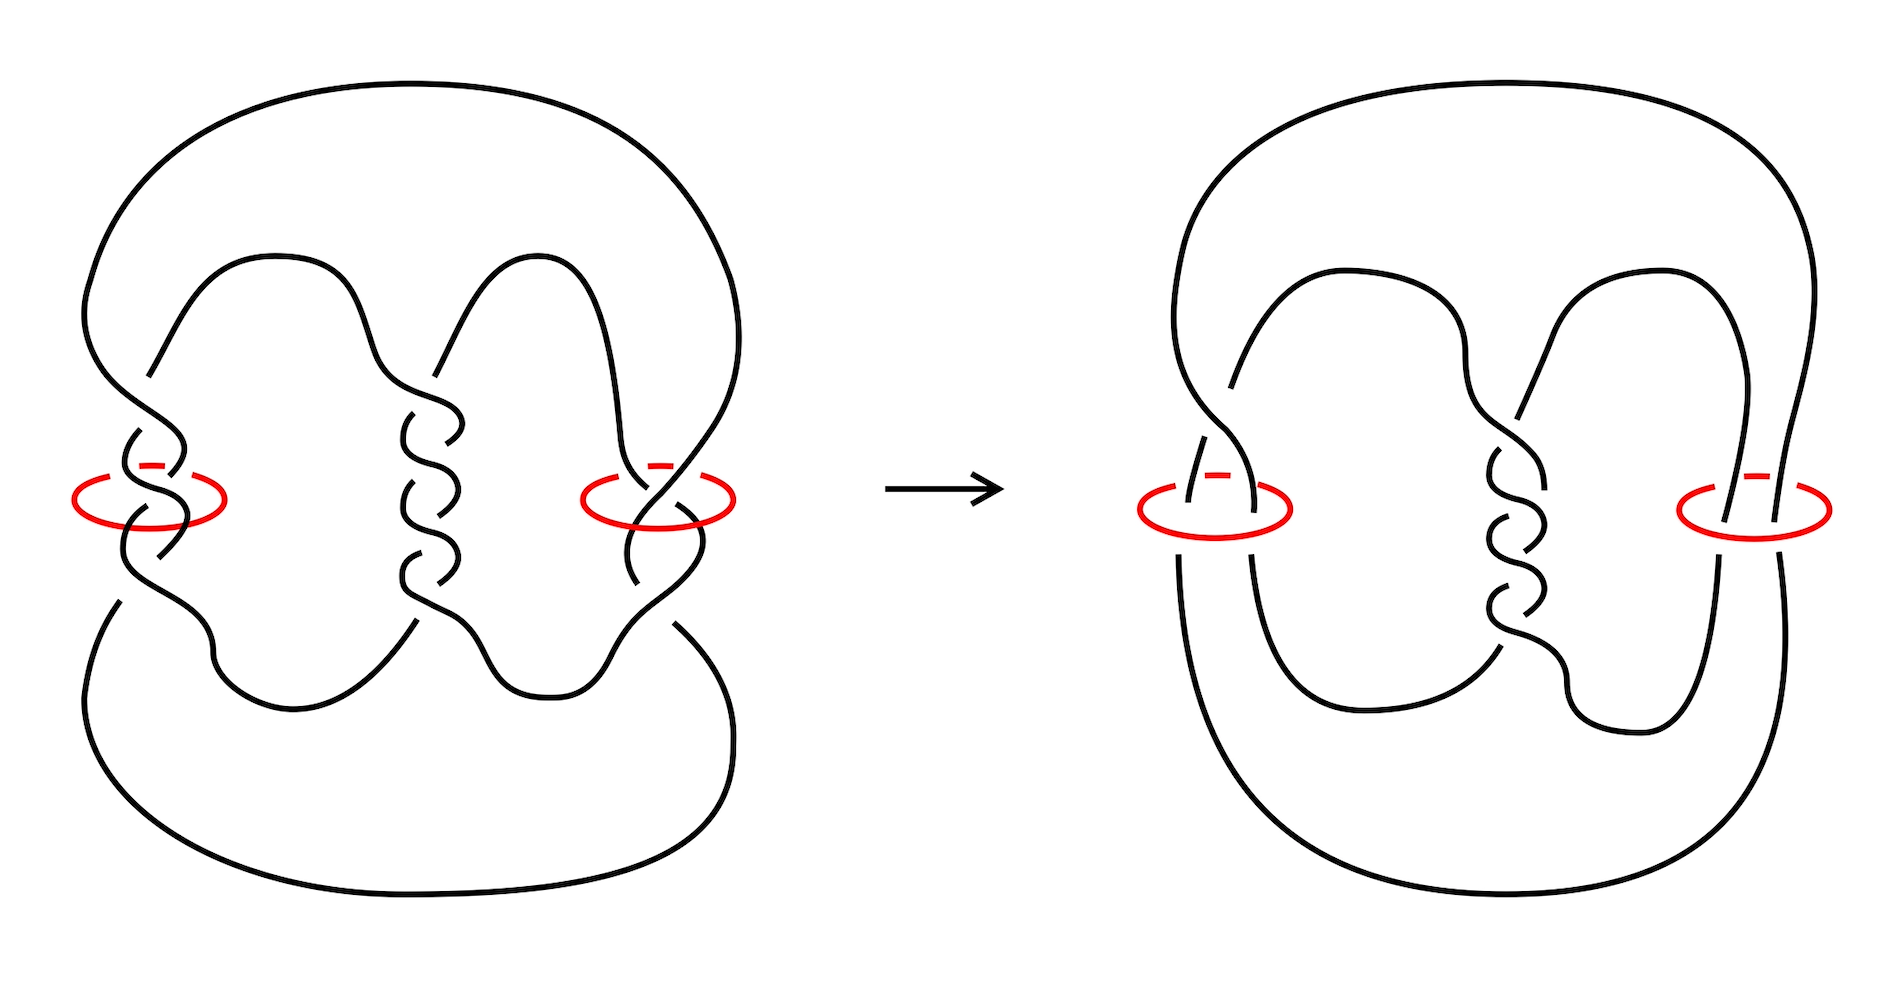
\includegraphics [height=4cm]{augmentation2}\\
  (a)&(b)
  \end{tabular}
 \caption{The left shows a pretzel knot before augmentation and the right shows after augmentation}
 \label{fig:augmentationS3}
 \end{figure}
 
 
 %%%%%%%%%%%%%%%%%%%%%%%%%%%%%%%%%%%%%%%%%%%%%%%%%%%%%%%% 
\section{Augmented Links}
 Champanerkar, Kofman and Purcell have studied alternating links in the thickened torus. They define a link in the thickened torus as a quotient of a biperiodic alternating link as follows,
 
\begin{define}\cite{CKP2}
\label{def:biperiodiclink}
A \emph{biperiodic alternating link} $\mathcal{L}$ is an infinite link
which has a projection onto
$\R^2$ which is invariant under an action of a two dimensional lattice $\Lambda$
by translations, such that $L=\mathcal{L}/\Lambda$ is an alternating link in
$\torus \times I$, where $I = (-1,1)$, with the projection on $\torus \times \{0\}$.
We call $L$ a link diagram in $\torus \times I$.   
\end{define}

\begin{remark}
Since $\torus \times I \cong \Sp^3 - H$, where $H$ is a Hopf link. The complement $\torus \times I- L = \Sp^3 - (L \cup H)$.
\end{remark}

Champanerkar, Kofman and Purcell \cite{CKP2} extended the definition of prime links in $\Sp^3$ for links in $\torus \times I$ called weakly prime. 

 \begin{define} \label{def:weaklyprime}
A diagram of a link $L$ is weakly prime if whenever a disk is embedded in the diagram surface meets the diagram transversely in exactly two edges, then the disk contains a simple edge of the diagram and no crossings.
\end{define}


\begin{define}
A \emph{twist region} in a link diagram $L=\mathcal{L}/\Lambda$ in $\torus \times I$, is the quotient of a twist region in the biperiodic link $\mathcal{L}$. %a string of bigons, or a single crossing in the diagram on the universal cover of $\torus \times I$ is called a . 
A biperiodic link $\mathcal{L}$ is called \emph{twist-reduced} if for any simple closed curve on the plane that intersects $\mathcal{L}$ transversely in four points, with two points adjacent to one crossing and the other two points adjacent to another crossing, the simple closed
curve bounds a subdiagram consisting of a (possibly empty) collection of bigons
strung end to end between these crossings. We say $L$ is \emph{twist-reduced} if it is the quotient of a twist-reduced biperiodic link. 
\end{define}

Now we can define augmentation for a link in $\torus \times I$ the same way we define augmentation for links in $\Sp^3$. For a link in $\torus \times I$, the crossing circles are added to the diagram projected onto $\torus \times \{0\}$. Let $L$ be a twist reduced diagram in $\torus \times I$, we define {\it augmentation} as a process in which an unknotted circle component is added to one or more twist regions of $L$. See Figure \ref{fig:Augmentations}


 \begin{figure}
 \centering
 \begin{tabular}{cccc}
 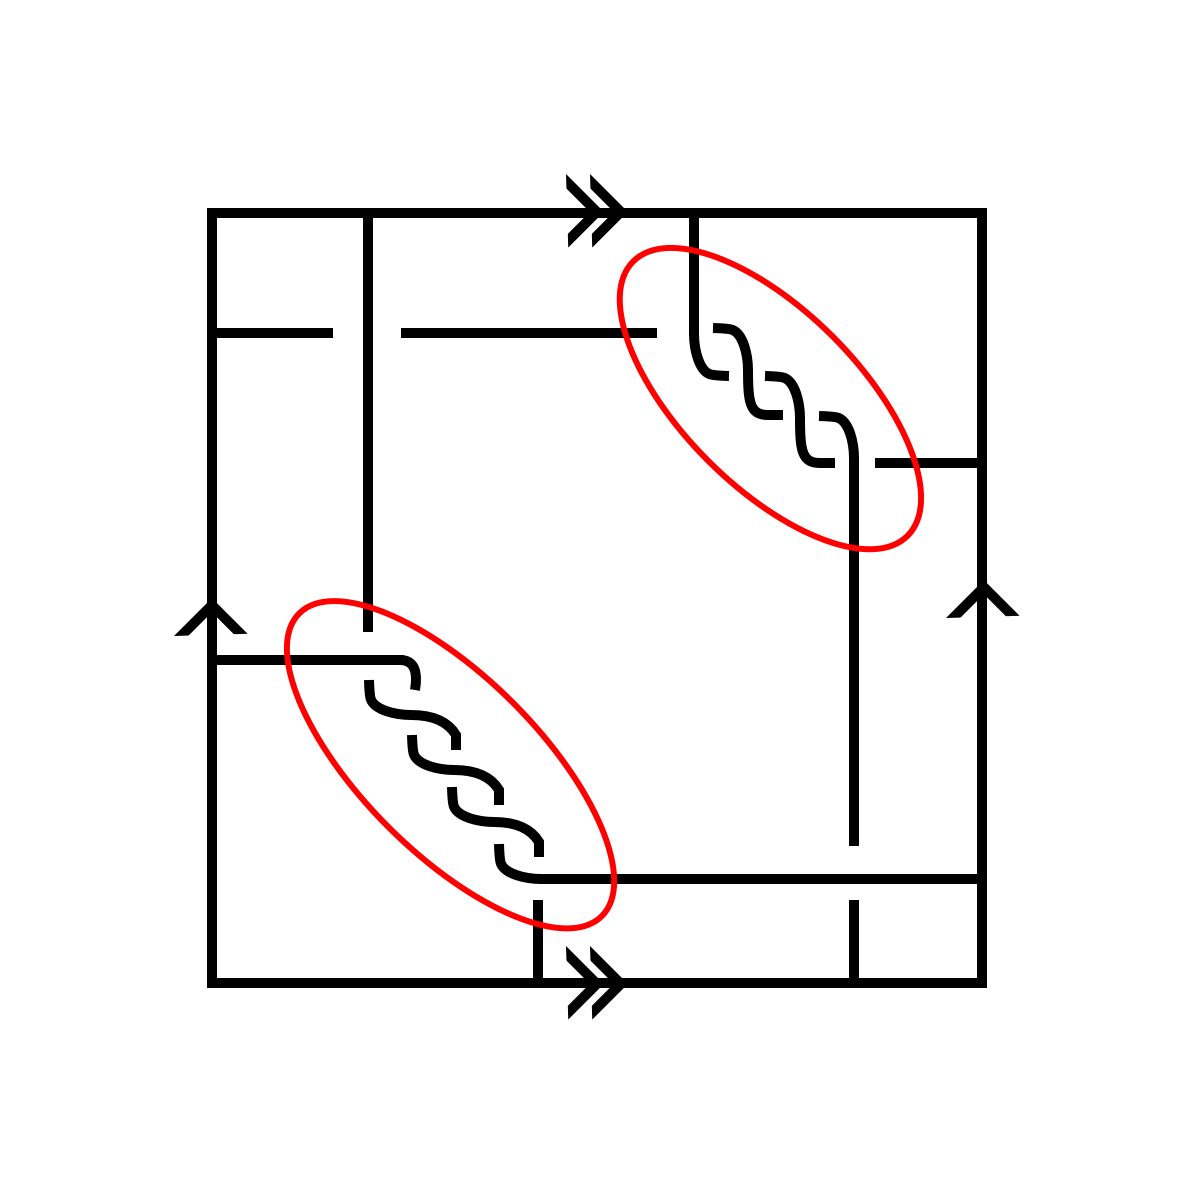
\includegraphics [width=3cm]{fig1}&
 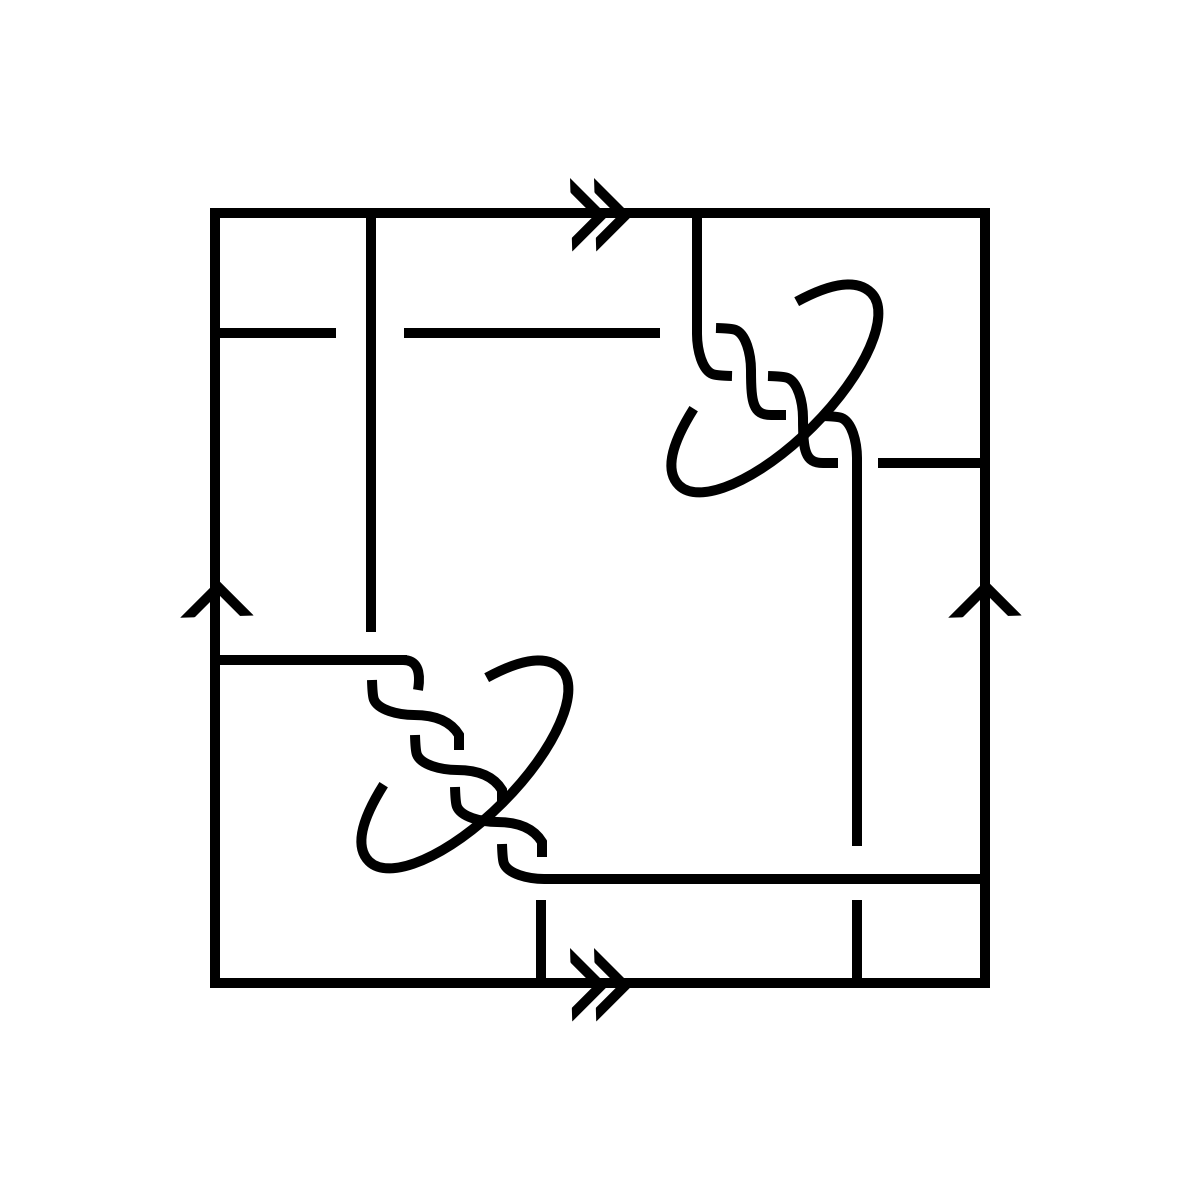
\includegraphics  [width=3cm]{twist-augment}&
  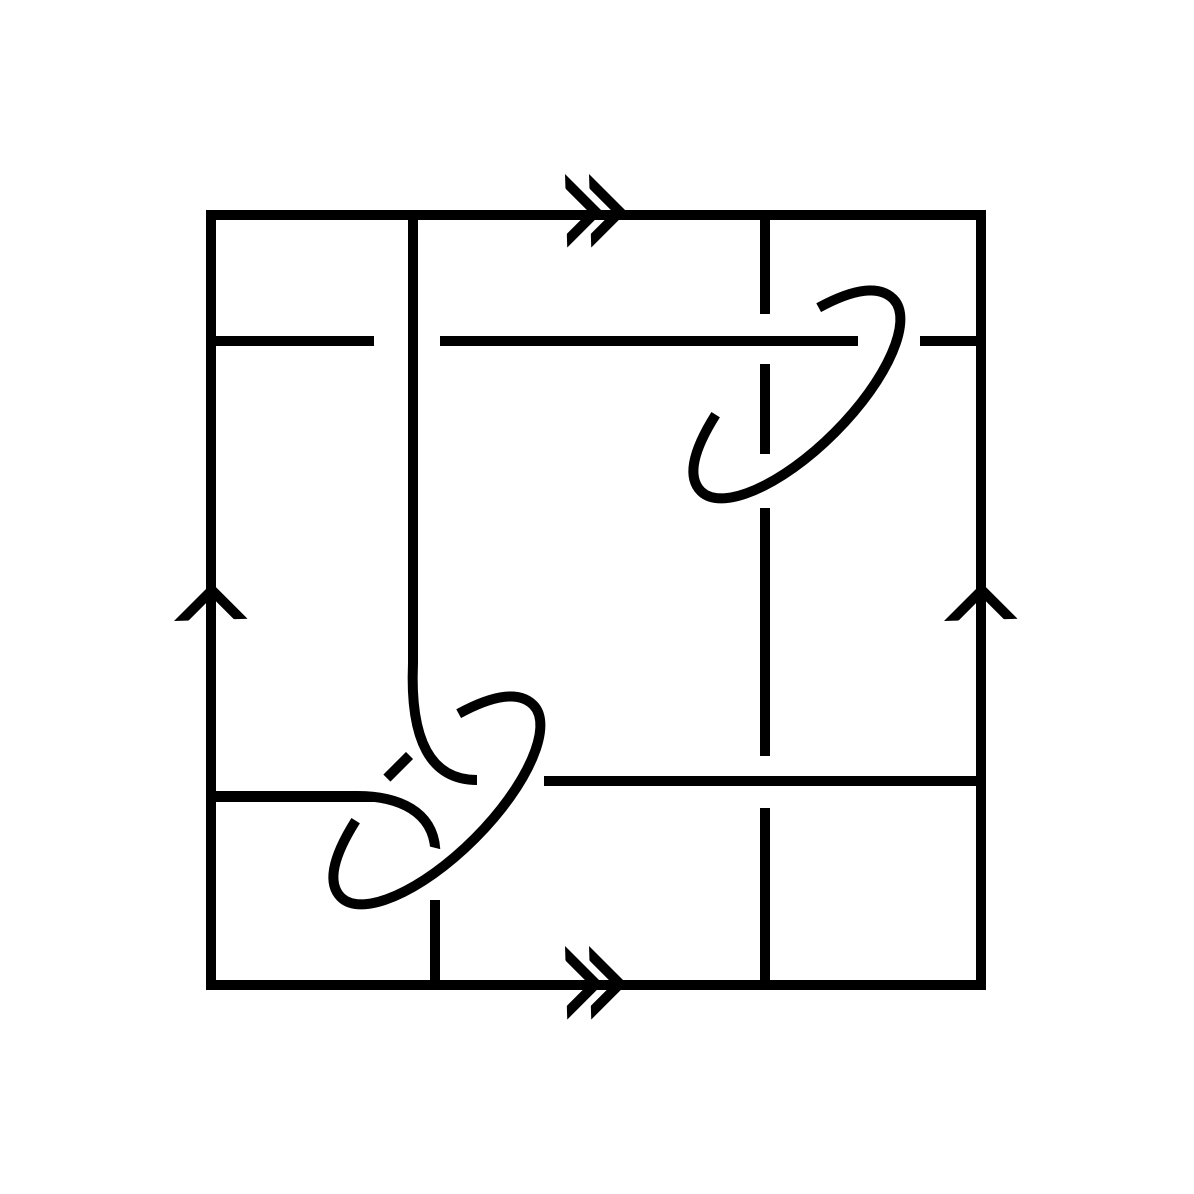
\includegraphics [width=3cm]{fig-2}\\
 % 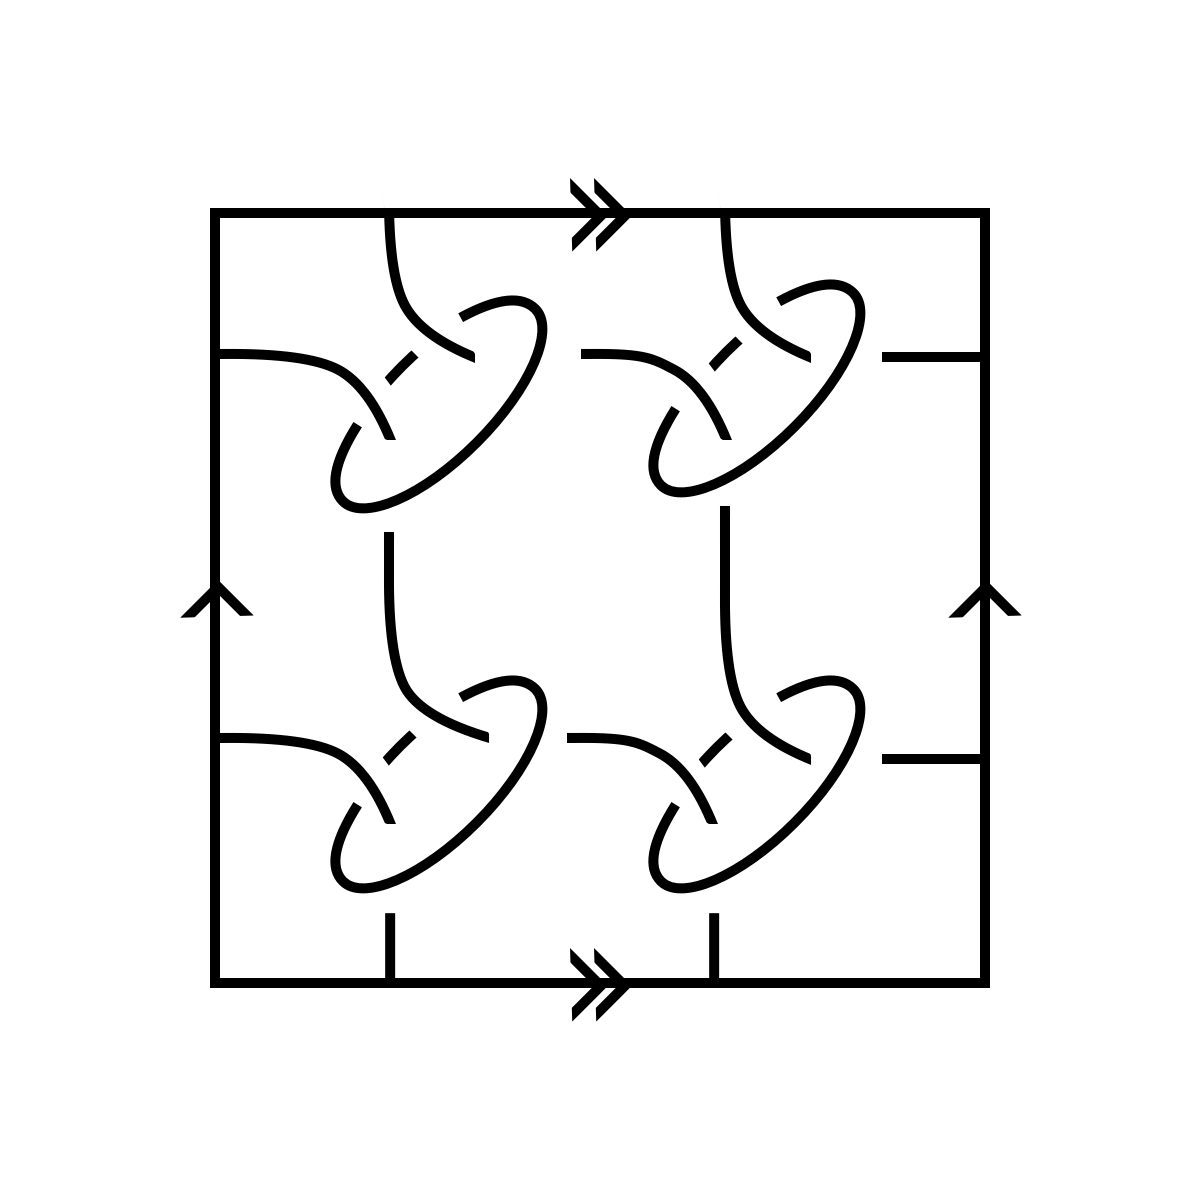
\includegraphics [width=3cm]{fal}\\
  A&B&C
  \end{tabular}
 \caption{A: The top right has an odd number of twists while the bottom left has an even number of twists. B: The picture of the link on the right after augmentation twist regions circled in red. C: The link with the twists removed.}
 \label{fig:Augmentations}
 \end{figure}
%%%%%%%%%%%%%%%%%%%%%%%%%%%%%%%%%%%%%%%%%%%%%%%%%%%% 

\subsection{Torihedral Decomposition of Augmented Alternating Links in Thickened Torus}


We show a method of decomposing an augmented link in the thickened torus into
two torihedra. The idea is to combine methods of Menasco
\cite{Menasco} and the use of crossing edges between each crossing of our link
and Lackenby's ``cut-slice-flatten" method \cite{lackenby} on the augmentation
sites.   


\begin{define}\cite{CKP2}
\label{def:torihedron}
A \emph{torihedron} $\sT$ is a cone on the torus, 
i.e. $\torus \times [0,1]/(\torus \times \{1\})$, with a cellular graph
$G = G(\sT)$ on $\torus \times \{0\}$.
An \emph{ideal torihedron} is a torihedron with the
vertices of $G$ and the vertex $\torus \times \{1\}$ removed. Hence, an ideal
torihedron is homeomorphic to $\torus \times [0,1)$ with a finite set of points
(ideal vertices) removed from $\torus \times \{0\}$.
We refer to the vertex $\torus \times \{1\}$ as the cone point.
\end{define}


For visualization purposes, we typically draw the graph $G(\sT)$ of a
torihedron from the perspective of the cone point $\torus \times \{1\}$.

If the faces of $G(\sT)$ are disks,
then $\sT$ can be decomposed into a union of pyramids,
obtained by coning each face to the cone point of $\sT$.
This also gives a decomposition of the corresponding ideal torihedron
into ideal pyramids.
We call these the \emph{pyramidal decompositions} of $\sT$ and its
ideal version.


\begin{prop}\label{p:tori_decomp}
Let $L$ be an augmented link in $\torus \times I$.
%Let $G(L)$ be a diagram of the link on $\torus \times \{0\}$.
There is a decomposition of the complement,
$(\torus \times I) - L$ into two ideal torihedra.
\end{prop}

\begin{proof}
We will begin by assuming that there are no half twists and then
arrange the link diagram of $L$ in the following way: first place the added
circle components (augmentation) perpendicular to the projection plane, $\torus
\times \{0\}$ leaving the remaining part of the link parallel to the projection
plane.  We now place a crossing edge on each crossing of the link so that for
each crossing edge, one end of the edge lies on a bottom strand while the other
end lies on a top strand as in Figure \ref{fig:crossingArc} left.

\begin{figure} \centering 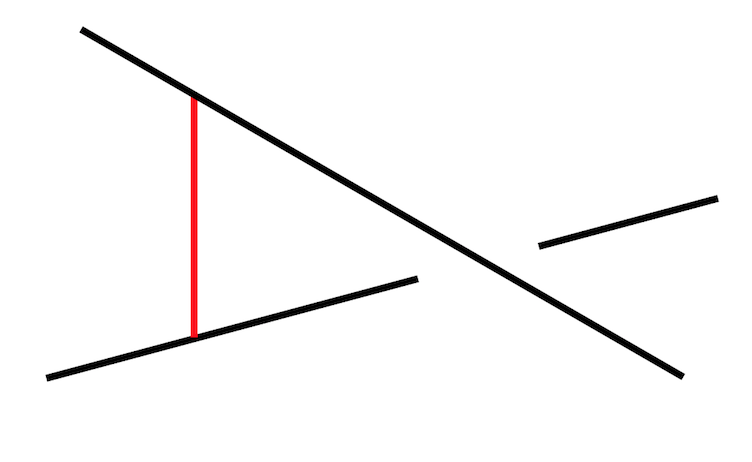
\includegraphics[width=4cm]{crossingArc}
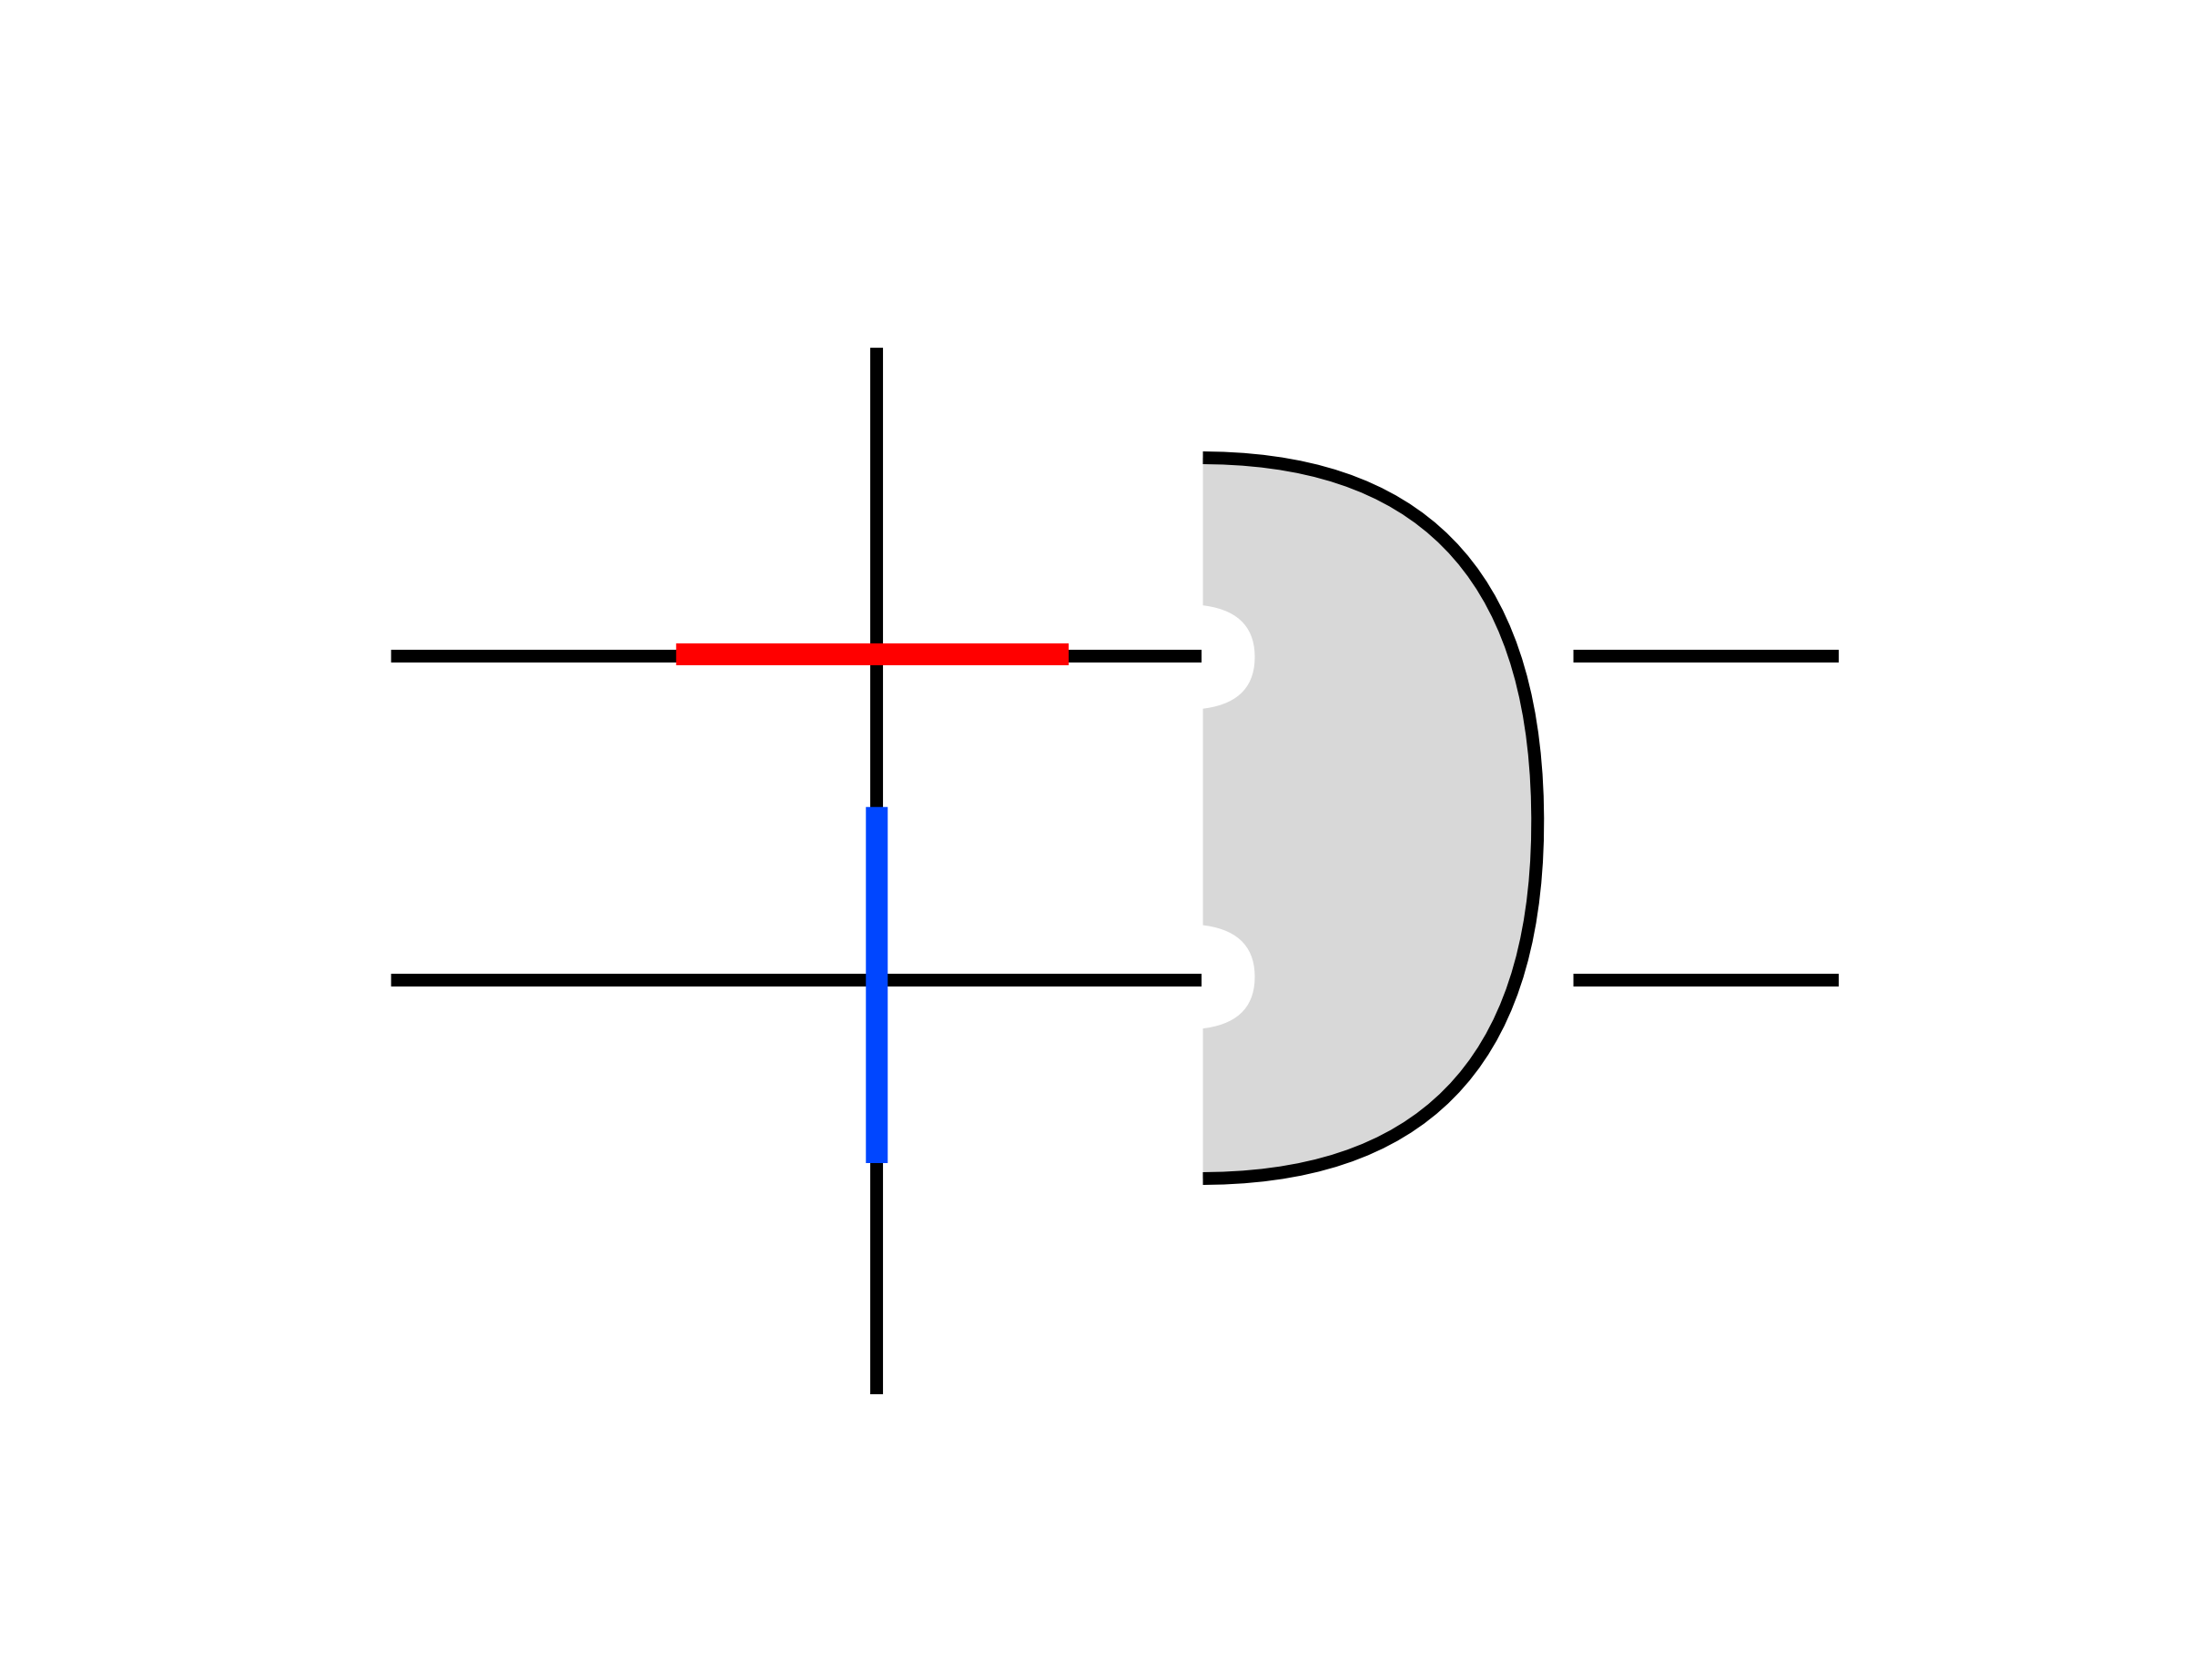
\includegraphics[width=5cm]{crossingPush} \caption{Left: The black strands are
part of the link and the red strand is the crossing edge. Right: The blue and
red edges represent the split crossing edges and the shaded half disk is bounded
by the crossing circle} \label{fig:crossingArc} \end{figure}

\indent We view the link from the point at infinity from the top. We will push
the top strand to the bottom strand, splitting the crossing edge into two
identical edges as in Figure \ref{fig:crossingArc} right. We push the link
components to infinity and stretch the crossing edge so that we have flattened
the link onto $\torus \times \{0\}$ except for the crossing circles which will
remain perpendicular to the projection plane. 
 
\indent Now place a disk on each crossing circle, so that the disk is bounded by
the crossing circle. We can then cut $\torus \times I$ along $\torus \times \{0\}$ and
focus on the top half, $\torus \times [0,1)$. We will follow the same method on the
bottom half to obtain the second identical torihedron. The disk we place on each
crossing circle is now cut in half. This half disk is now bounded by the
projection plane and the semi-cricle arc of the crossing circle. We push down on
the crossing circle and split the disk into two identical disks. We then push
the arc of each crossing circle to infinity, collapsing them to ideal vertices.
We obtain two triangular faces which represent the disk which look like a
bow-tie as in Figure \ref{fig:falGluings}. 

\begin{figure}
 \centering
 \begin{tabular}{cc}
 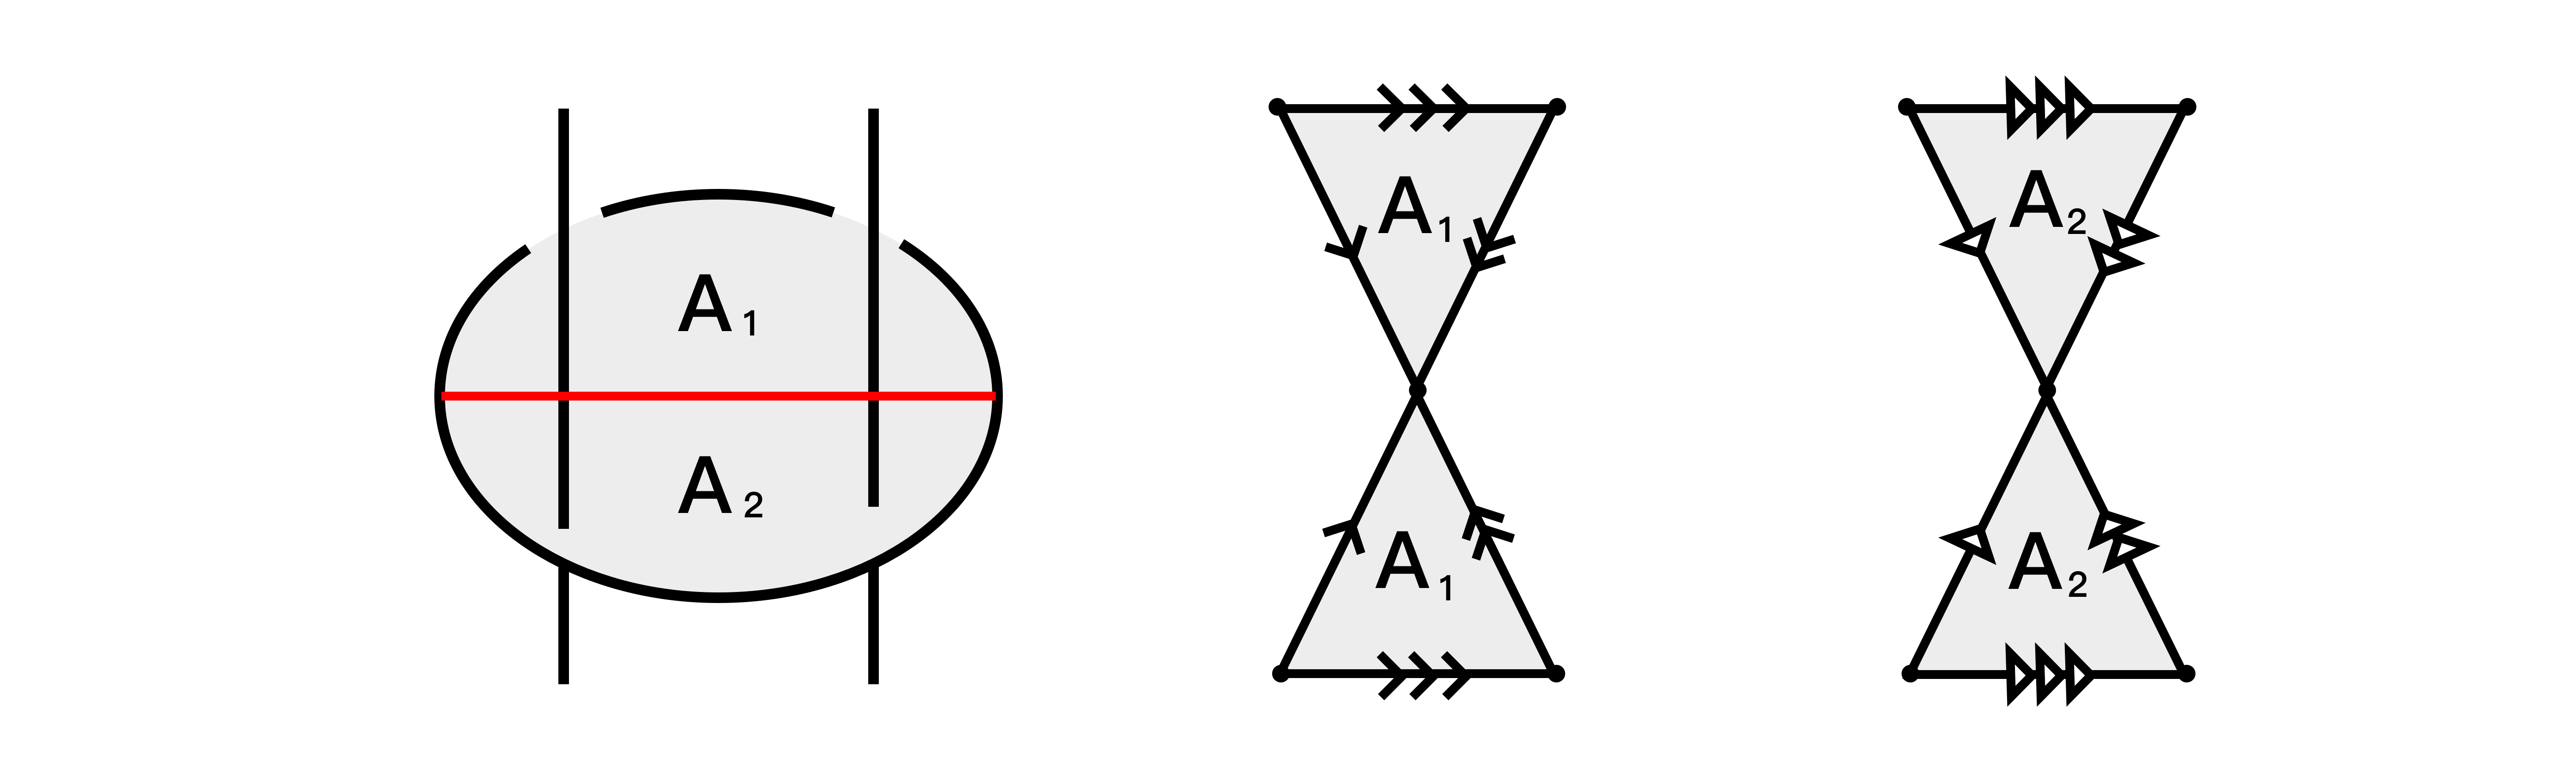
\includegraphics [width=8cm]{falGluing1}&
 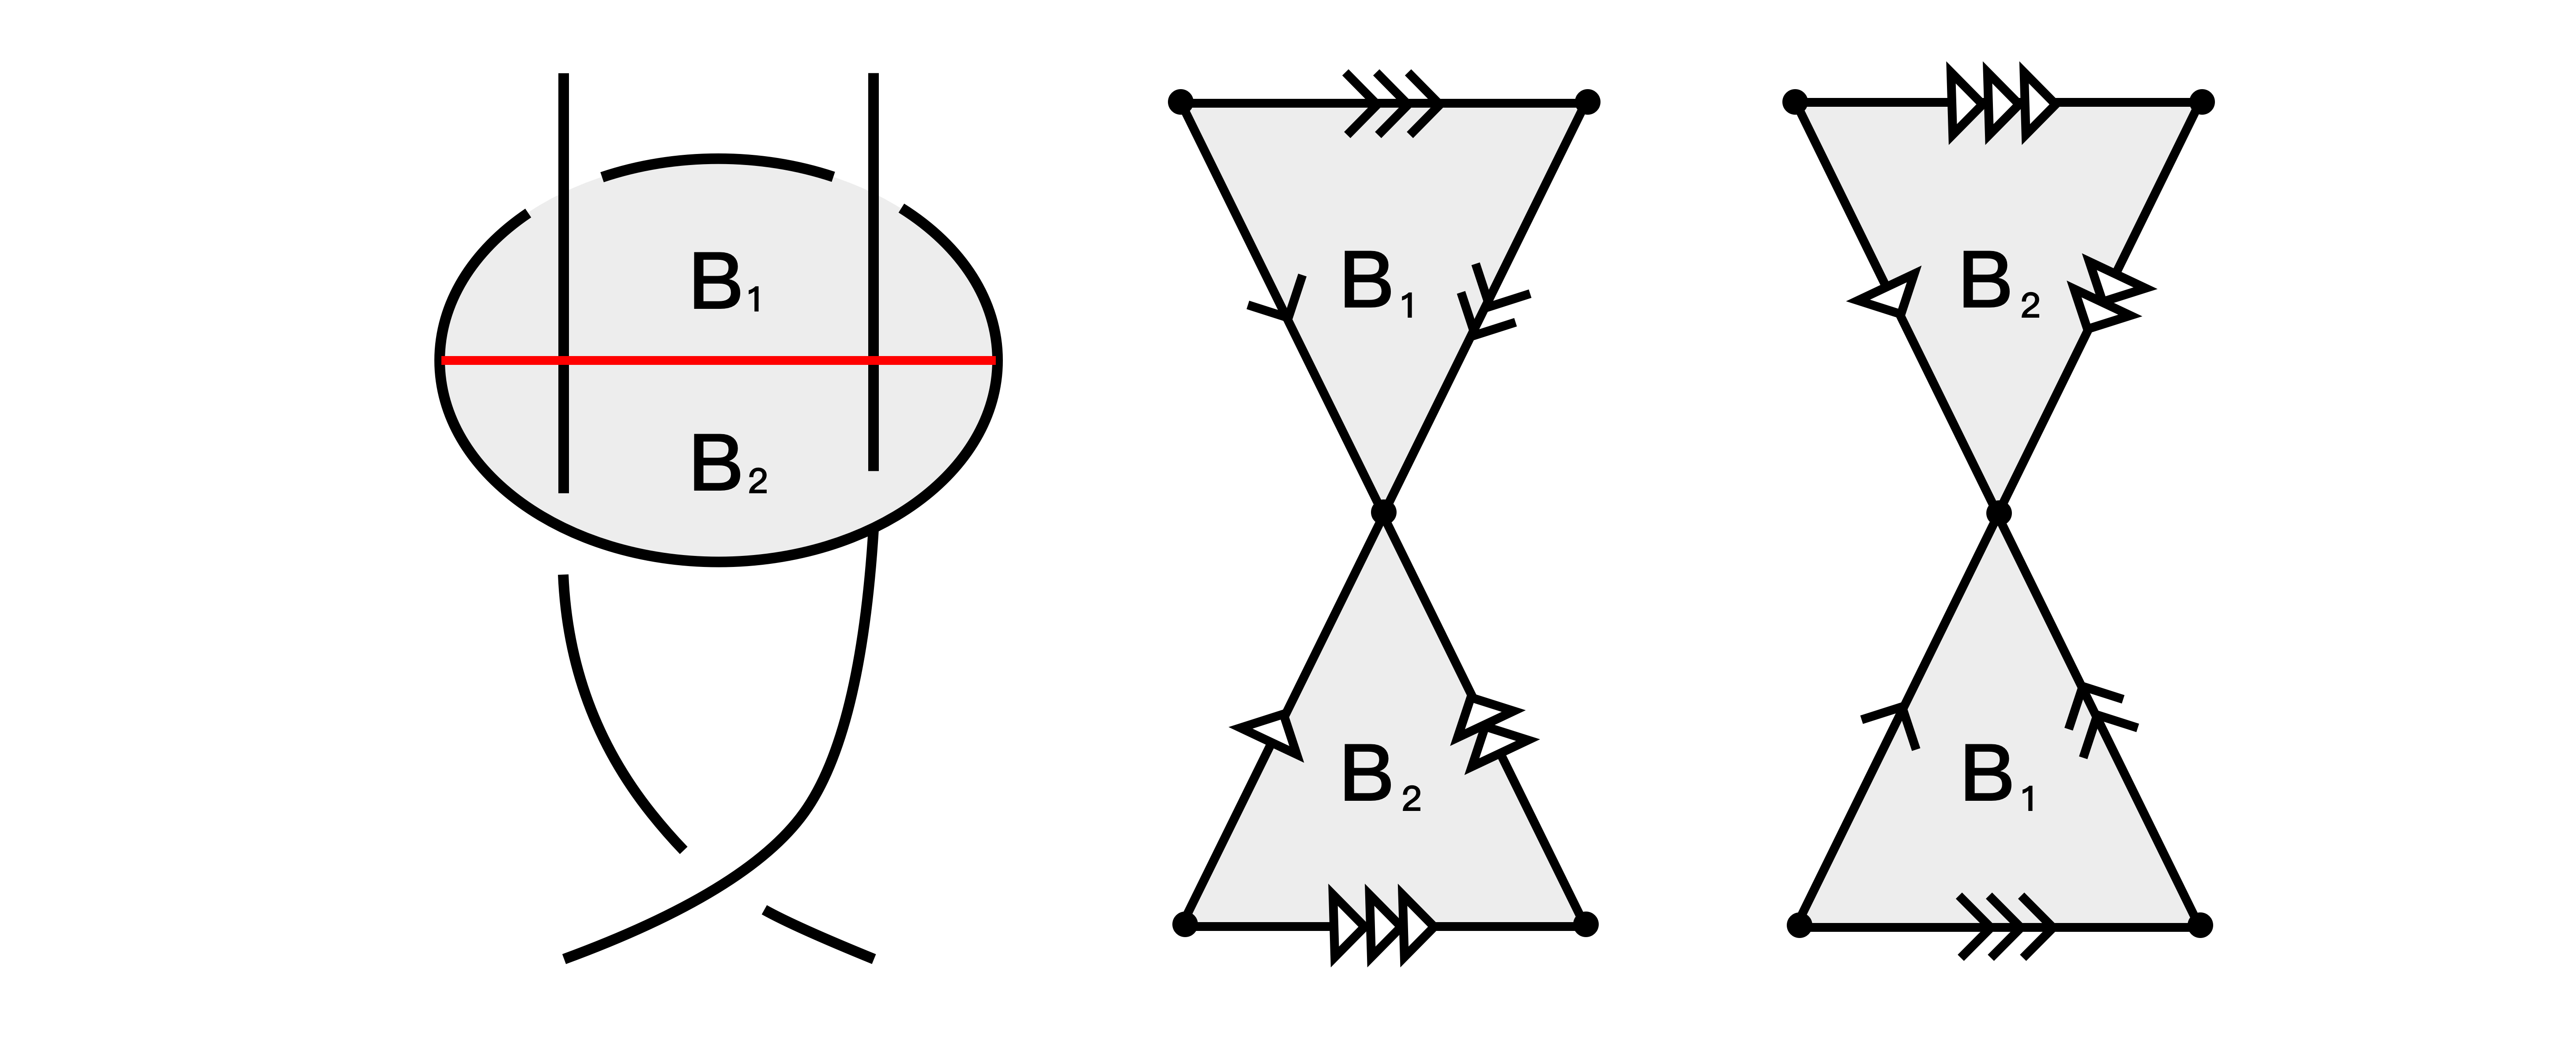
\includegraphics [width=7cm]{falGluing2}\\
 (a)&(b)
 \end{tabular}
 \caption{The first pictures shows gluing without half-twists the second shows gluing with half-twists}
 \label{fig:falGluings}
 \end{figure}

\indent We repeat the steps for the bottom half of $\torus \times I$, $\torus \times
(-1,0]$. Then we get two torihedra. The graph of each will come from
crossing edges and edges of the disk. Now, if there are half twists we will
decompose the complement of the link the same way as if there are no half twists
and we will identify the two bow-ties as in Figure \ref{fig:falGluings}.
Finally,
we obtain the complement of the link by gluing the two torihedra with the gluing
information given by identifying crossing edges and triangles of the bow-tie. We
glue the faces of the torihedra which do not correspond to a bow-tie with a
$2\pi/n$ twist where $n$ is the number of sides of each face as in Figure
\ref{fig:top-bottom} clockwise or counterclockwise.


For future reference, we will denote the graph for the top and bottom
torihedra by $\Gamma_T(L)$ and $\Gamma_B(L)$, respectively,
where both graphs are viewed from the cone point of the top torihedron
$\torus \times \{1\}$.
Note that if $L = K$ is the non-augmented link,
$\Gamma_T(L)$ is simply the link projection $K$,
and in fact $\Gamma_T(K) = \Gamma_B(K)$.

\end{proof}


%%%%%%%%%%%%%%%%%%%%%%%%%%%%
The following figures is an example which decomposes the link (C) of Figure
\ref{fig:Augmentations}.  \begin{figure}[h] \centering 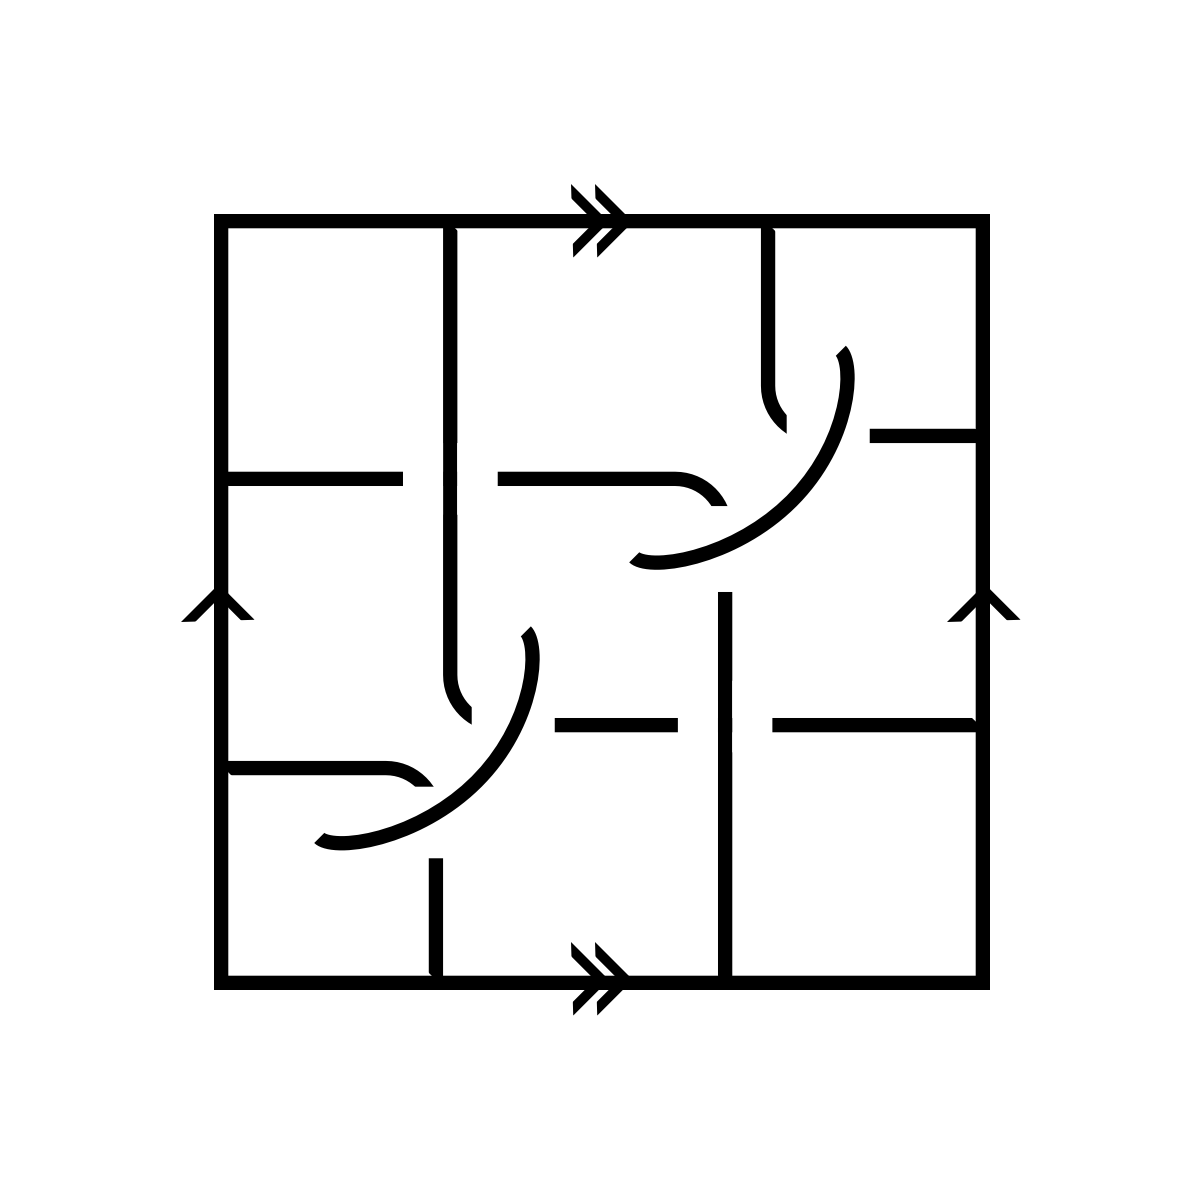
\includegraphics
[height=3cm]{fig-3} 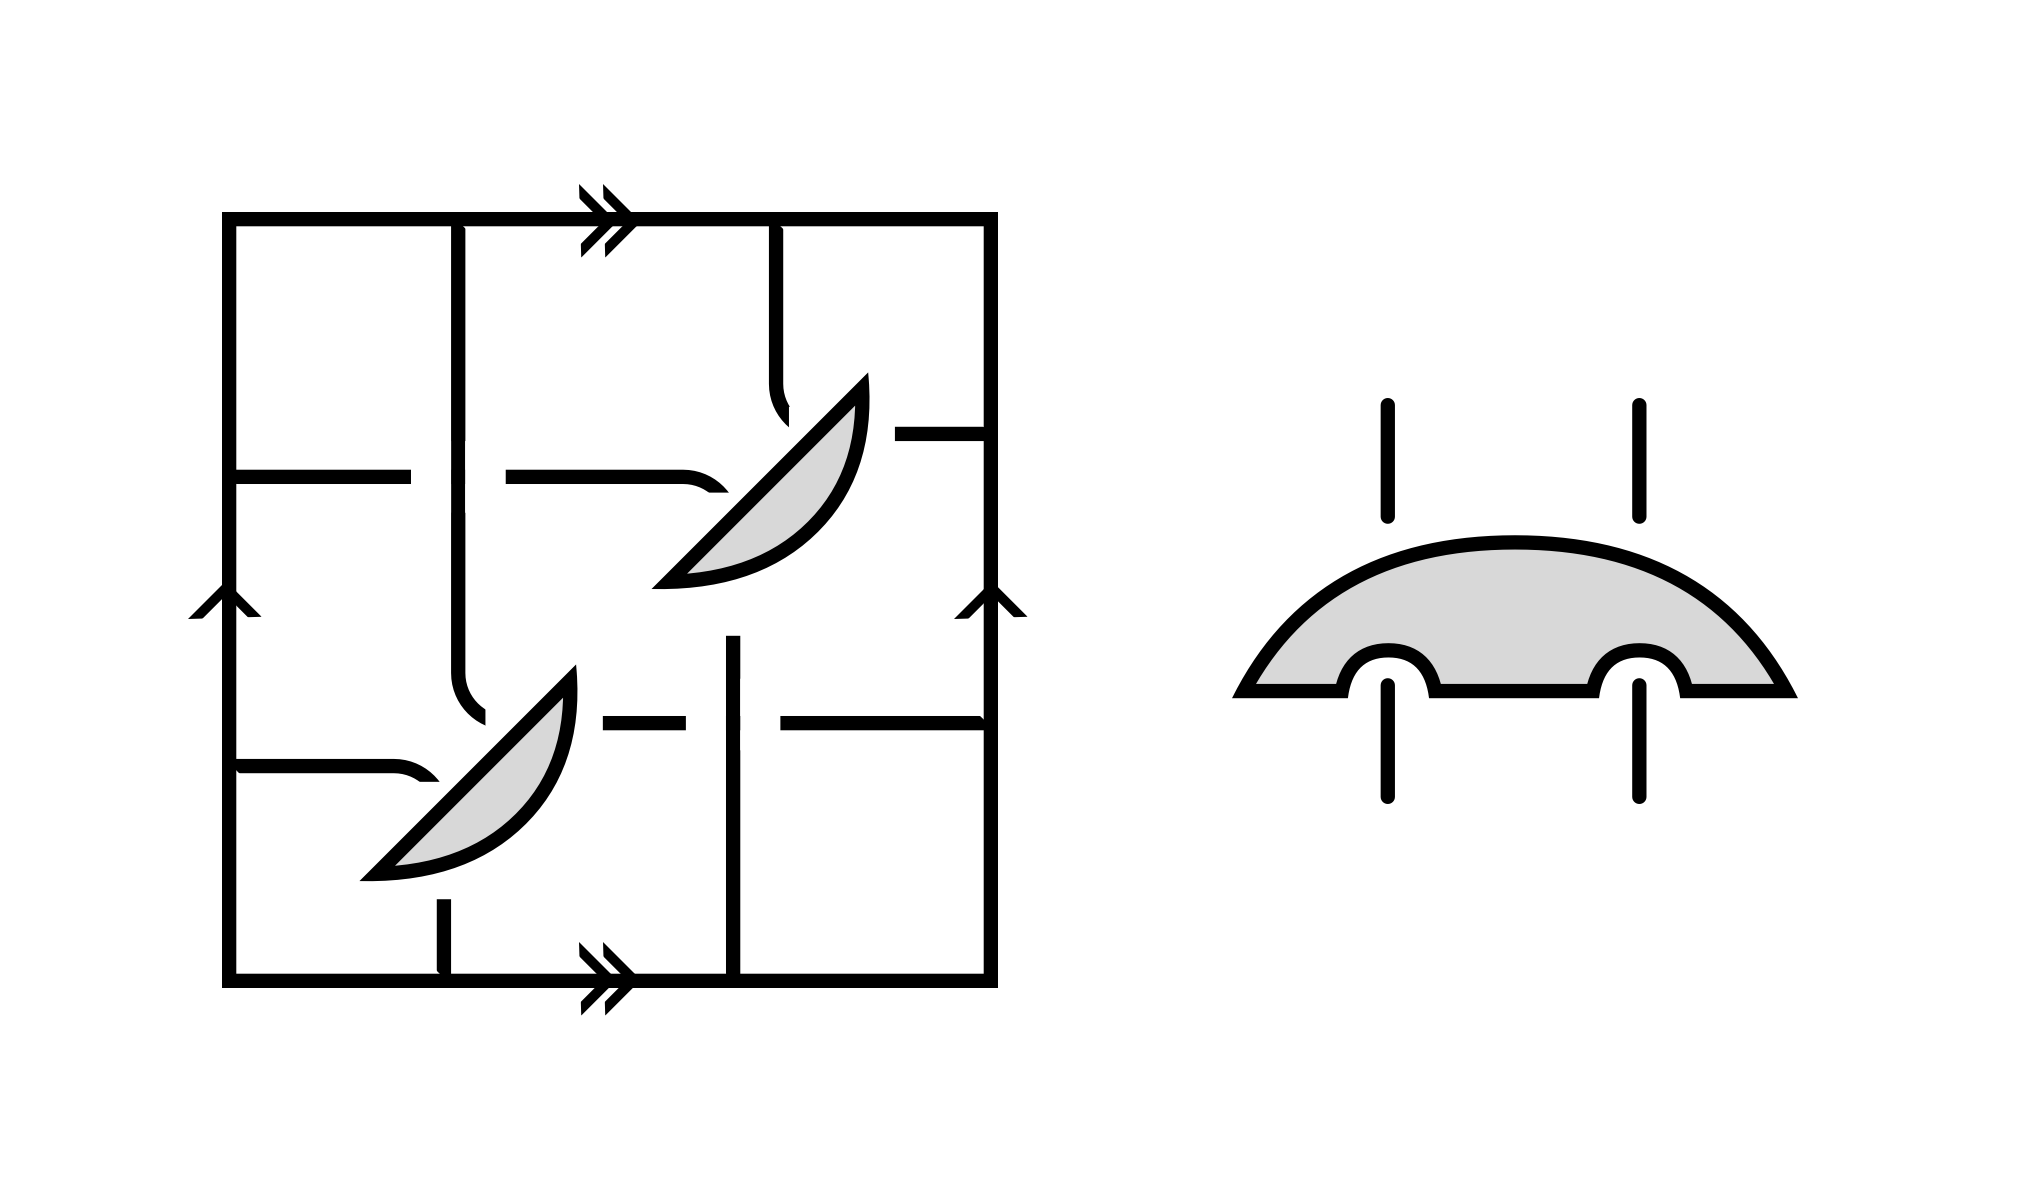
\includegraphics [height=3cm]{fig-4} \caption{Each crossing
circle bounds a disk} \end{figure}
 
 \vspace*{-0.5cm} \begin{figure}[h] \centering 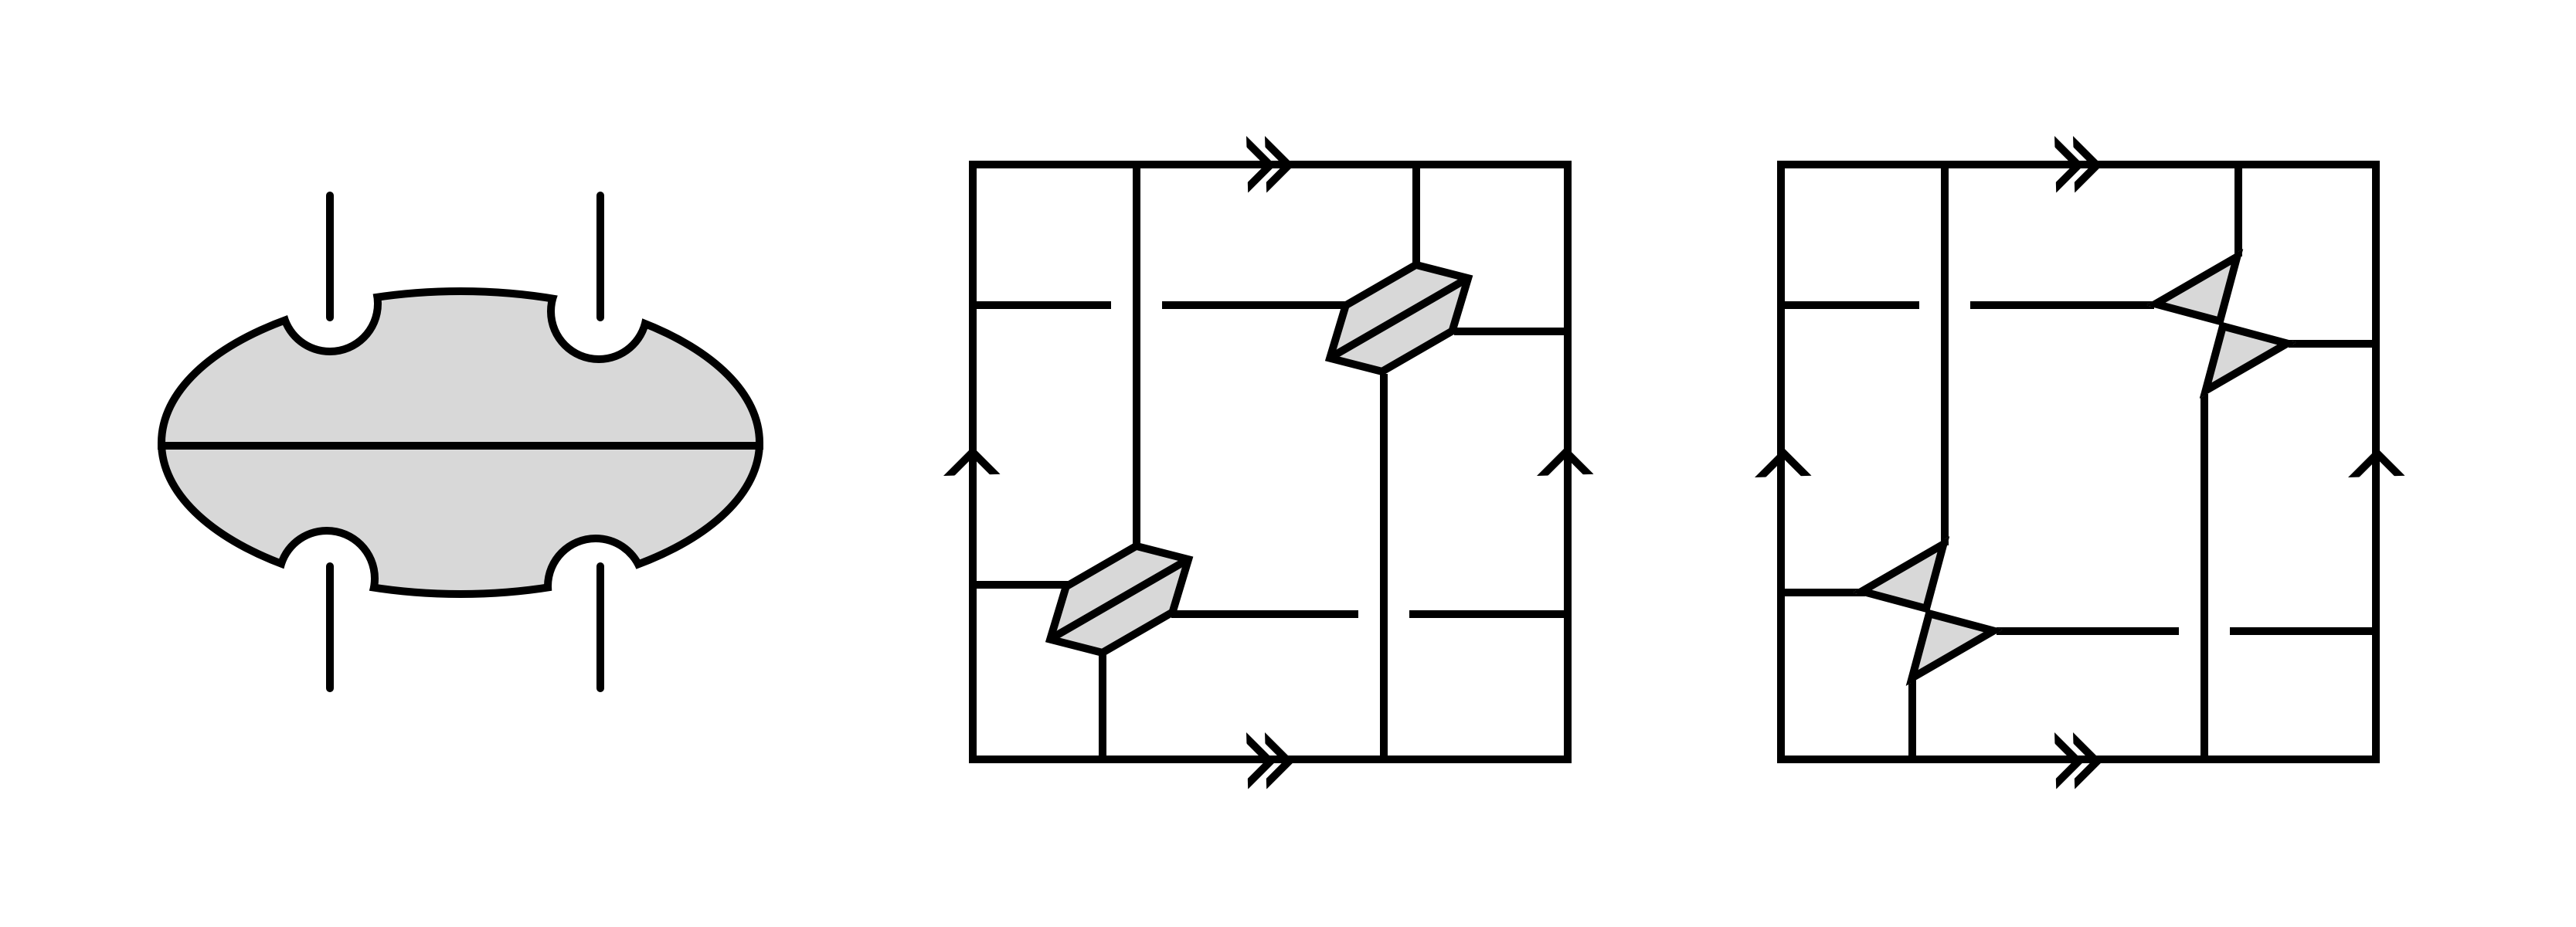
\includegraphics
 [height=3cm]{fig-5} \caption{We split the disk and collapse the arc of each
 crossing circle to ideal vertices} \end{figure}
 
	\vspace*{-0.5cm} \begin{figure}[h] \centering 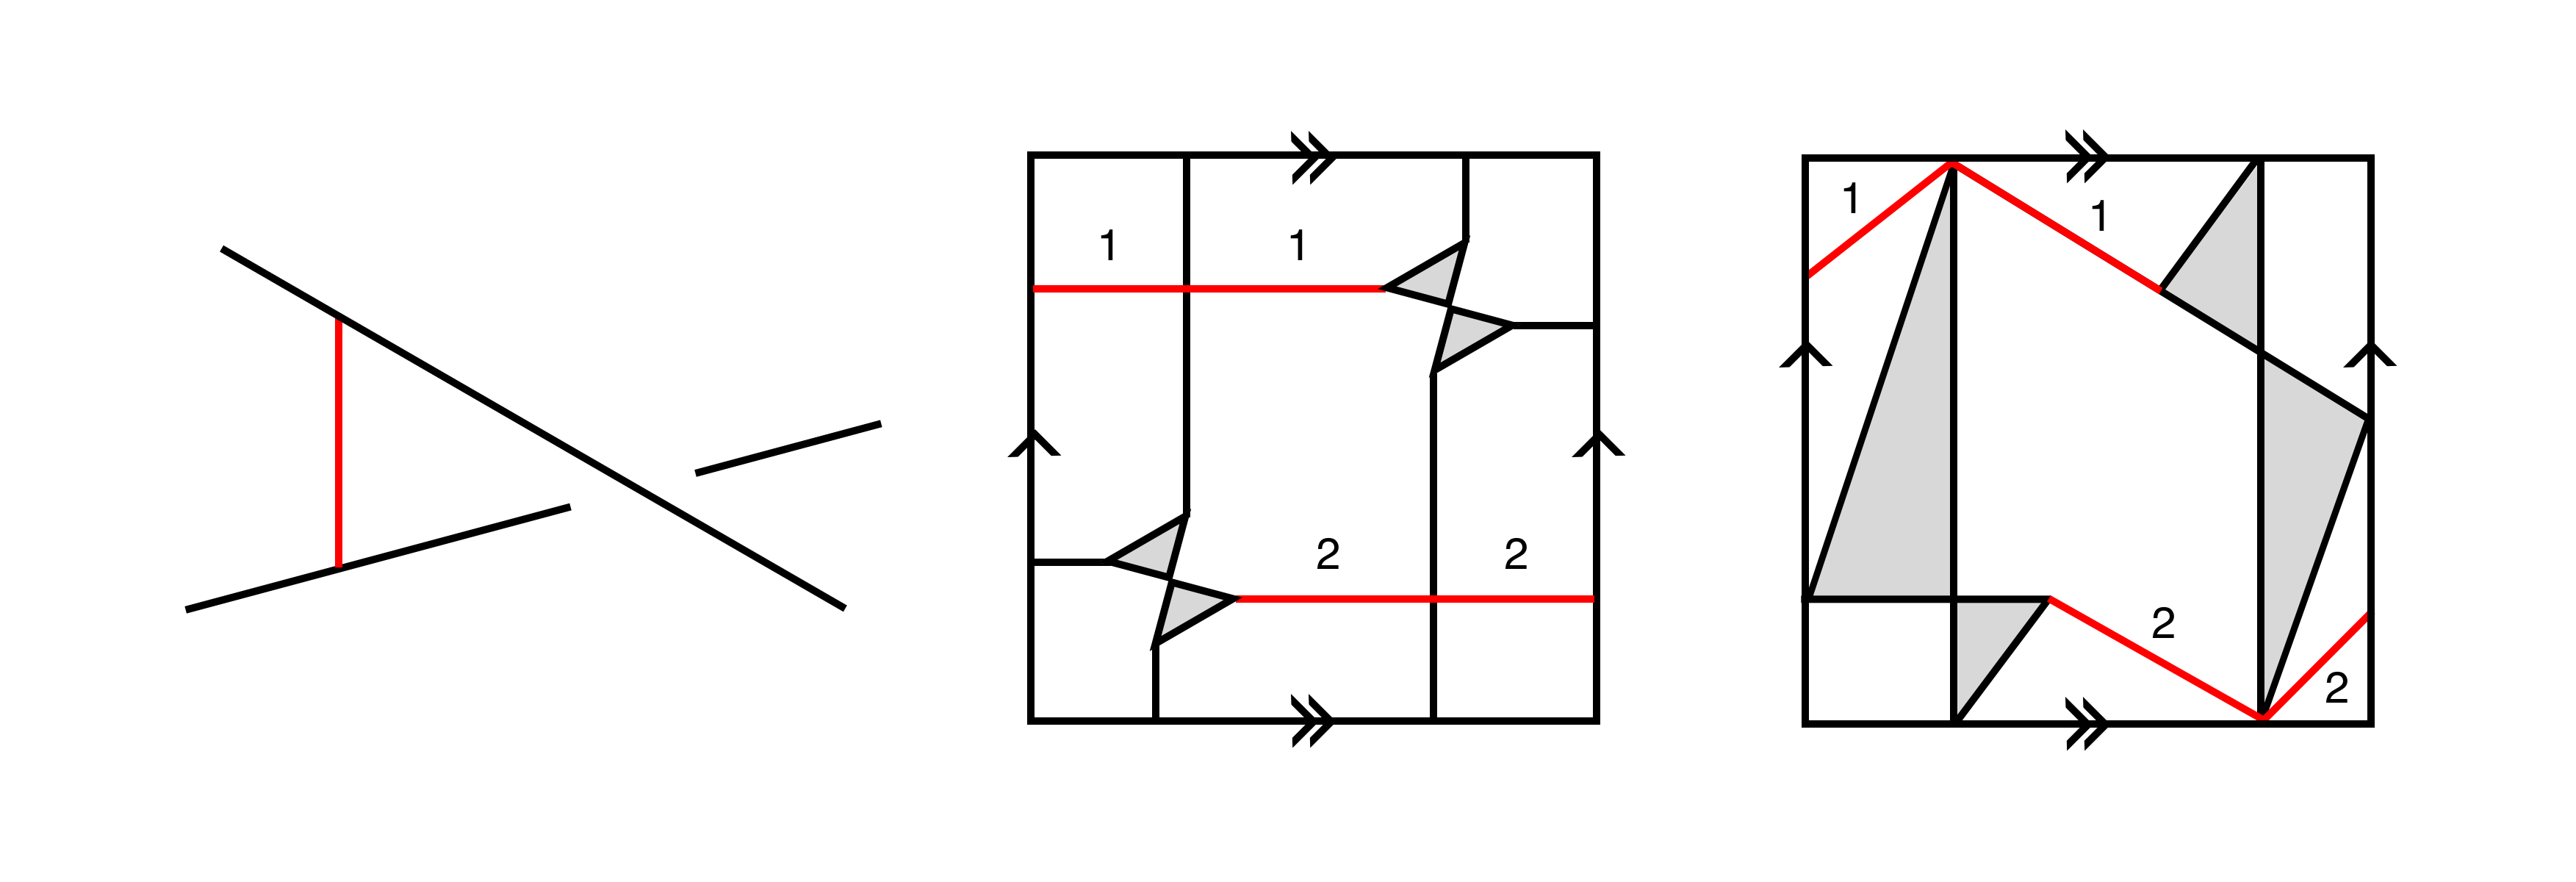
\includegraphics
	[height=3cm]{fig-6} \caption{Left: The crossing arc is the edge in red.
	Middle: Picture of splitting the crossing edge. Right: The link component is
	pushed off to infinity.} \end{figure}

 \vspace*{-0.5cm} \begin{figure}[h] \centering 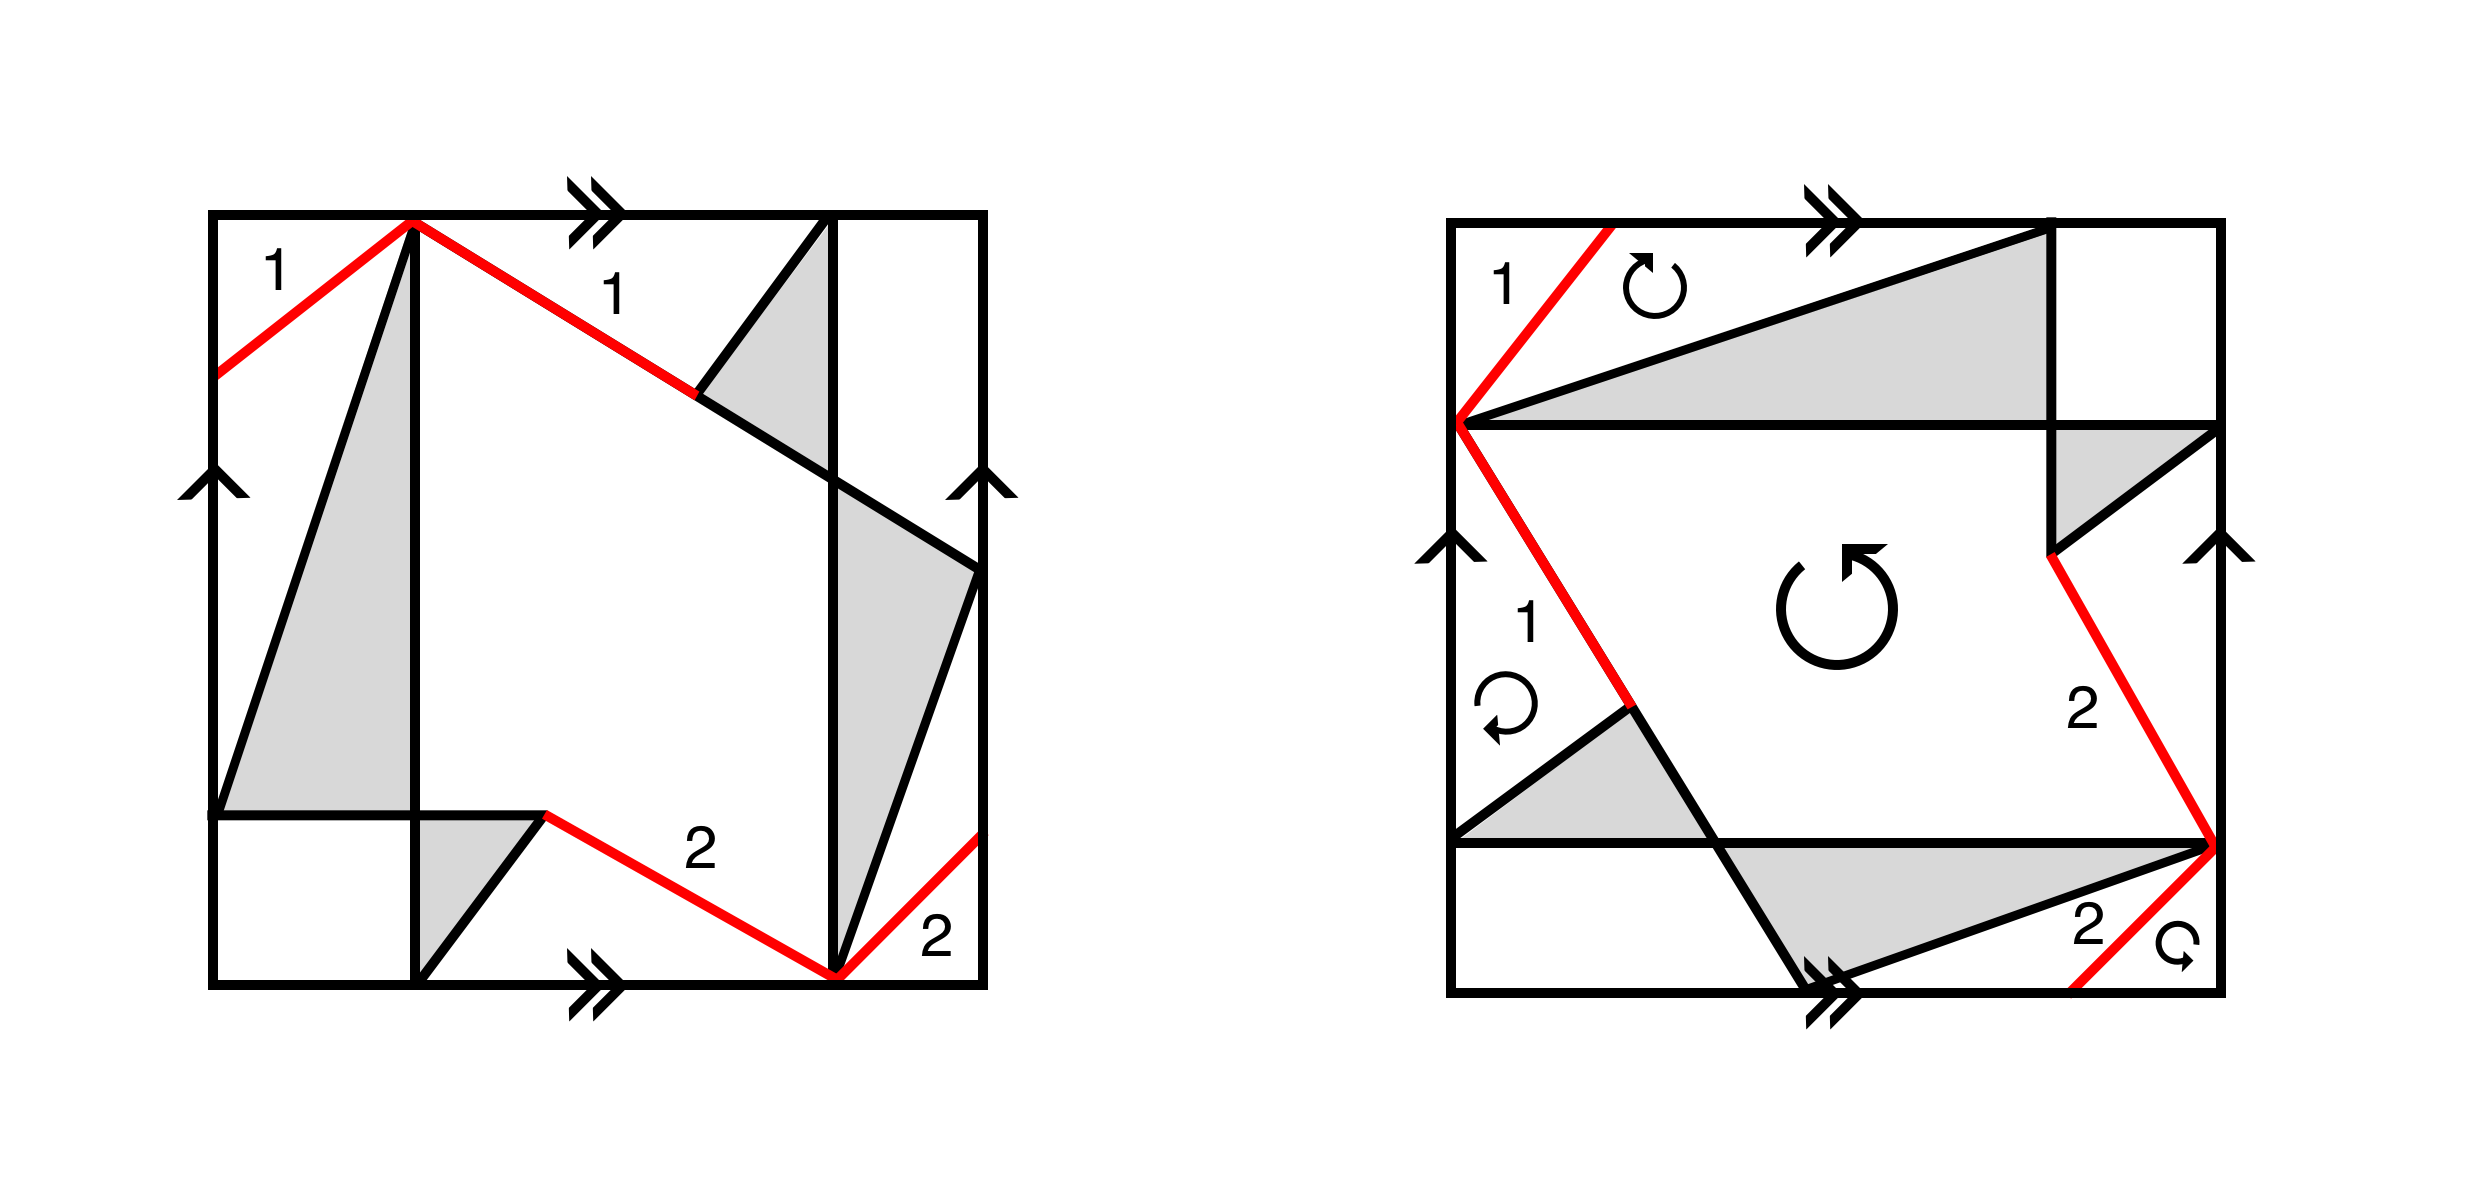
\includegraphics
 [height=3cm]{top-bottom} \caption{
	Left: The top torihedron.
	Right: The bottom torihdron with rotation for face gluing.} \label{fig:top-bottom} \end{figure}


\comment{
\begin{remark}\label{cor:triangulation}
The faces of one torihedron which do not correspond to a bow-tie glue to a
corresponding face of the second torihedron to form bipyramids. One can add
stellating edges, edges which have vertices corresponding to the different
components of the Hopf link that cuts through the center of the face to
decompose the bipyramids into tetrahedra. This process is called {\it
stellation}. Stellating all the bipyramids of the decomposition obtained from
Proposition \ref{p:tori_decomp} we obtained a triangulation of the
complement of $L$ which is made up of {\it horizontal} edges (edges from the
graph of the torihedra), {\it vertical} edges (edges from coning vertices of the
the graph of the torihedra) and stellating edges.
\end{remark}
}

\comment{
\begin{proof}[Proof of Remark 2.7]
Using the decomposition from Proposition
\ref{p:tori_decomp} we can add a stellation edge whose end points
are $\torus \times \{-1\}$ and $\torus \times \{1\}$ which cut through faces of $\torus \times I$ which do not come from the augmentation disks like in \cite{CKP2}.
Since each face of the top torihedron gets glued to the bottom torihedron, we
obtain bipyramids, and the stellation edge will decompose the bipyramids into
tetrahedra. Then the link of the vertex  $\torus \times \{1\}$ or
$\torus \times \{-1\}$ is the graph of the torihedron
%$\torus \times [0,1)$ or
%$\torus \times (-1,0]$ respectively.
\end{proof}
}


TODO refer to BS about theta's
\begin{definition}
An \emph{angled torihedron} $(\sT, \theta_\bullet^*)$
is a torihedron $\sT$ with
an assignment $\theta_e^* \in [0,\pi]$
such that for each vertex $v \in G(\sT)$,
$\sum_{e \ni v} \theta_e^* = (\deg(v) - 2)\pi$.
We also denote $\theta_e = \pi - \theta_e^*$,
so $\sum_{e \ni v} \theta_e = 2\pi$;
we refer to $\theta_e$ as the exterior angle
and $\theta_e$ as the interior angle.


We say $(\sT, \theta_\bullet^*)$ is \emph{degenerate}
if $\theta_e^* = 0$ for some edge;
we say it is \emph{non-degenerate} otherwise.
\end{definition}


One may ask for the pyramidal decomposition of a torihedron
to ``respect" angles. The following definitions make sense of this.

\begin{define}
An \emph{angled ideal tetrahedron} is an ideal tetrahedron with an assignment of a dihedral angle
to each edge, such that
\begin{itemize}
\item each dihedral angle is in $[0, \pi]$;
\item for each tetrahedron, opposite edges have equal dihedral angles;
\item the three distinct angles sum to $\pi$.
\end{itemize}

We say a angled ideal tetrahedron is \emph{degenerate} if
one dihedral angle is 0; we say it is \emph{non-degenerate} otherwise.
\end{define}


\begin{define}
A \emph{base-angled ideal pyramid}
is a pyramid whose base is an $n$-gon, $n \geq 3$,
and each boundary edge $e_i$ of the base face is assigned a dihedral angle
$\alpha_i \geq 0$ such that the sum is $\sum \alpha_i = 2\pi$.
The vertical edge $e_i'$ that meets $e_i$ and $e_{i+1}$
is automatically assigned the dihedral angle $\pi - \alpha_i - \alpha_{i+1}$.


We say a base-angled ideal pyramid is \emph{degenerate} if
$\alpha_i = 0$ for some $i$; we say it is \emph{non-degenerate} otherwise.
\end{define}


Clearly, the dihedral angles of an ideal hyperbolic pyramid
make it a base-angled ideal pyramid
(with $\alpha_i = \vphi_{e_i}$);
it is not hard to see that the converse is true:
simply consider a circumsribed polygon such that the side $e_i$
subtends an angle of $2\alpha_i$ at the center,
and take the ideal hyperbolic pyramid over it in upper-half space.
Also, an angled ideal tetrahedron is simply a base-angled ideal pyramid
with base a triangle, and with no preferred face.

\begin{definition}
%TODO: this definition should come after base-angled pyramid
An \emph{angle splitting} of an angled torihedron $(\sT,\theta_\bullet^*)$
is a splitting of $\theta_e^* = \vphi_{\vec{e}} + \vphi_{\cev{e}}$
for each edge $e$,
such that for each face $f$,
$\sum_{\vec{e} \in \del f} \vphi_{\vec{e}}^* = \pi$.

Equivalently, an angle splitting is a decomposition of
$\sT$ into base-angled pyramids,
one for each face of $G(\sT)$, such that
for each boundary edge $e$ of $\sT$,
the dihedral angles from the two adjacent pyramids
add to $\theta_e^*$.
\end{definition}

TODO same as [BS] ``coherent angle system'' or something.


TODO check the feasible flow stuff.


\begin{lemma}
%Let $P_n$ be an ideal pyramid whose base is an $n$-gon and suppose,
%\begin{itemize}
%\item each boundary edge of the base face is assigned a dihedral angle $\alpha_i$ such that for adjacent edges, $\alpha_i + \alpha_{i+1} < \pi$;
%\item we are given a decomposition of the base face into triangles by adding new edges. 
%\end{itemize}
Let $P_n$ be a base-angled ideal pyramid, and suppose we are given a
decomposition of the base face into triangles by adding new edges.  One gets an
obvious corresponding triangulation of $P_n$, where a new face is added for each
new edge. Then there is an assignment of a dihedral angle to each edge of each
ideal tetrahedron in this triangulation such that
\begin{itemize}
\item each tetrahedron is an angled ideal tetrahedron;
\item the sum of dihedral angles around each new edge is $\pi$;
\item the dihedral angles of the edges of the original base face are the same as
	before.
\end{itemize} 
\end{lemma}

\begin{proof}
Induct on $n$; there is nothing to prove for the base case $n=3$.

The proof is essentially given in \figref{f:ideal_pyramid_arg} below

\begin{figure}
\label{f:ideal_pyramid_arg}
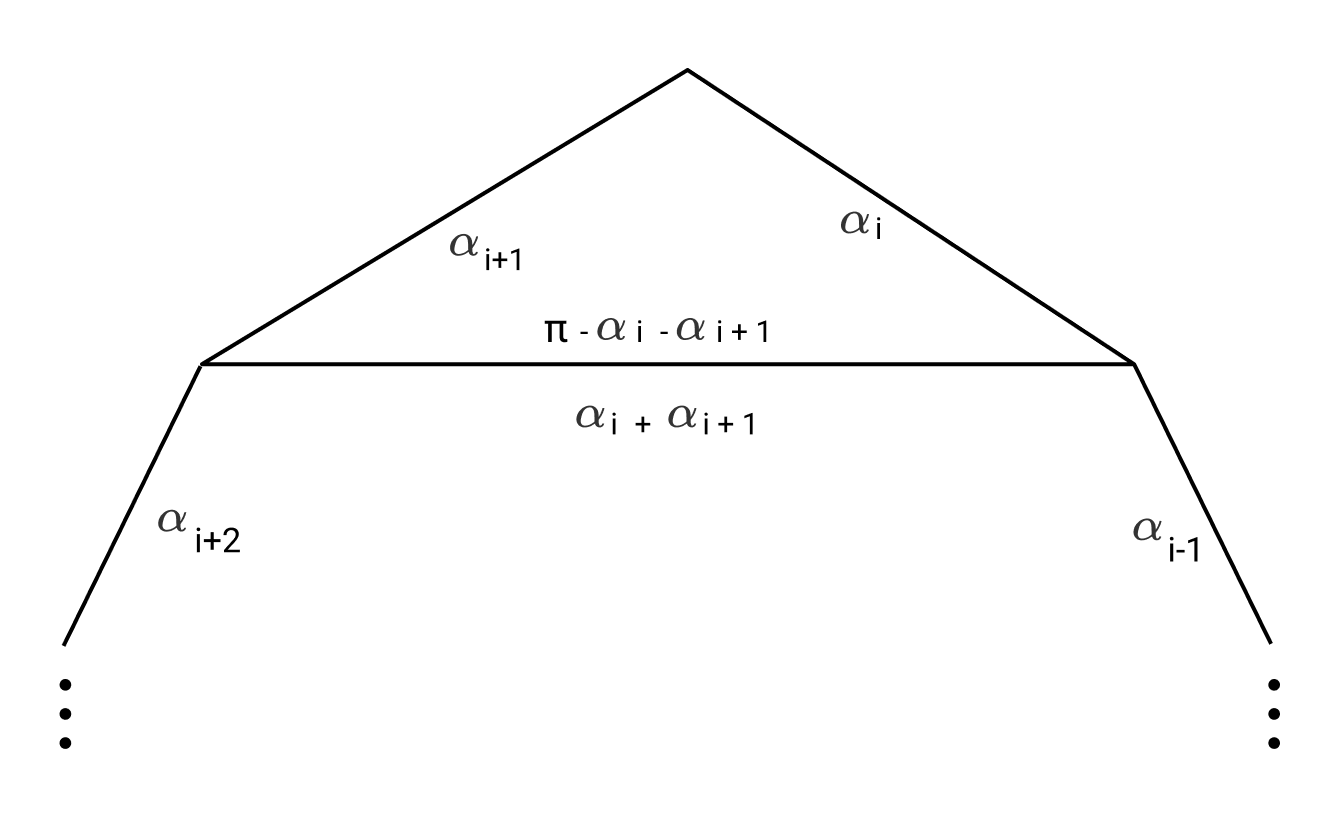
\includegraphics[height=8cm]{more_pictures/angle_split.png}
\end{figure}
Suppose the edges are labelled $e_i$,
which goes between vertices $v_i$ and $v_{i+1}$,
and suppose $e_i$ is assigned dihedral angle $\alpha_i$.
Let $e'$ be a new edge addeed to the base face of $P_n$
such that it separates the base face into a triangle and
an $(n-1)$-gon;
suppose the sides of the triangle are
$e_i, e_{i+1}$, and $e'$.
The new face corresponding to $e'$ separates $P_n$ into
an ideal tetrahedron $T$ and an ideal pyramid $P_{n-1}$.
We assign the dihedral angle of $\pi - \alpha_i - \alpha_{i+1}$
to $e'$ in $T$, and assign $\alpha_i + \alpha_{i+1}$ to $e'$ in $P_{n-1}$.
Clearly the sum of dihedral angles condition is satisfied
in $T$ and $P_{n-1}$.
It remains to check that the dihedral angles assigned to the vertical edges
are correct.
For the vertical edge associated to $v_j$ for $j \neq i, i+2$,
there is nothing to check;
for $j = i$, the dihedral angles are
$\pi - \alpha_i - (\pi - \alpha_i - \alpha_{i-1})$
in $T$ and $\pi - \alpha_{i-1} - (\alpha_i + \alpha_{i+1})$ in $P_{n-1}$,
which sum to $\pi - \alpha_i - \alpha_{i+1}$;
it is similar for $j = i+2$.

\end{proof}




%%%%%%%%%%%%%%%%%%%%%%%%%%%%%%%%%%%%%%%%%%%%%%%%%%%%%%%%%%%
\section{Hyperbolicity of Augmented Links}
Thurston introduced a method for finding the unique hyperbolic metric for a given 3-manifold $M$ with boundary consisting of tori \cite{Thurston}. The idea was to triangulate the interior of $M$ into ideal tetrahedra and give those tetrahedra hyperbolic shapes (called shape parameters) that glue up coherently in $M$. The shape parameter of a tetrahedron is described by the cross-ratio of its four vertices on the sphere at infinity. Thurston had written down a system of gluing equations with shape parameters whose solutions correspond to the complete hyperbolic metric on the interior of $M$. Casson and Rivin separated gluing equations into a linear and non-linear part \cite{Casson-Rivin}. Angle structures is the linear part of Thurston's gluing equations, and what we will use to attain hyperbolicity of complements of augmented links in the thickened torus. 

\begin{define}
Let $M$ be an orientable 3-manifold with boundary consisting of tori. An angle
structure on an ideal triangulation $\tau$ of $M$ is an assignment of a dihedral
angle to each edge of each tetrahedron, such that
\begin{itemize}
\item each tetrahedron is a non-degenerate angled ideal tetrahedron,
\item around each edge of $\tau$, the dihedral angles sum to $2\pi$.
\end{itemize}
\end{define}

\begin{theorem}\cite{Casson-Rivin}\label{thm:Casson-Rivin}
Let $M$ be a 3-manifold admitting an angle structure. Then $M$ is hyperbolic.
\end{theorem}

For a hyperbolic link $K$ in $\torus \times I$, we produce sufficient conditions
on augmentations such that the resulting link obtained from augmenting $K$ is
hyperbolic. The idea is to start with a graph from the torihedral decomposition
of the link $K$ which will give us a graph on each torihedron with $\pi/2$ edges
\cite{CKP2}. Then by results of \cite{BandS} there exist a corresponding
right-angled circle pattern. We then consider the augmented link $L$ and its
torihedral decomposition from Proposition \ref{p:tori_decomp} with a
corresponding ``degenerate" circle pattern. We deform this degenerate circle
pattern into a ``proper" circle pattern which will give us a polyhedral
decomposition of $(\torus \times I)-L$ with angles of the torihedra in our
torihedral decomposition. Which we can further decompose into tetrahedra with
angles satisfying conditions of an angle structure. 



\begin{define}
We say an augmentation is \emph{right-augmented} if, when both strands are
(locally) oriented such that they cross the augmentation disk in the same
direction, the crossing is positive/a right-handed half-twist.
See \figref{right_left_aug.png}.
We say an augmentation is \emph{left-augmented} if it is not right-augmented.
\begin{figure}
\label{f:right_left_aug}
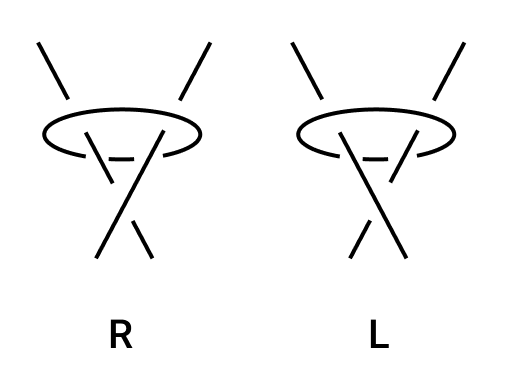
\includegraphics{more_pictures/right_left_aug.png}
\end{figure}
\end{define}

We can recover $L$ from the link diagram of $K$
together with labels at vertices indicating left- or right-augmentation.


\comment{
\begin{define}
Given a face $f$ of the original link diagram the \emph{augmentation sequence}
of $f$, denoted $\sigma_f$, is a cyclical sequence of symbols $0, L, R$ indexed
by vertices of $f$ going counter-clockwise, where, for $v \in \partial f$, the
$v$-th element is
\[
\sigma_f^v = 
\begin{cases}
0 \text{ if $v$ is not augmented} \\
L \text{ if $v$ is left-augmented} \\
R \text{ if $v$ is right-augmented}
\end{cases}
\]
\end{define}
}


\comment{

\begin{prop}
Suppose $L$ is obtained from augmenting $K$,
so that for each face $f$ of the link projection of $K$,
the augmentation sequence $\sigma_f$ has no $L$ adjacent to $R$.
Then the TODO CONTINUE HERE
\end{prop}
}

\comment{
\begin{prop}
Let $\Sigma$ be a closed surface with a cellular decomposition.
Suppose we have labelled some edges by either $`+'$ or $`-'$,
such that for each face $f$,
\begin{itemize}
	\item no two adjacent edges have the same label,
	\item the length of consecutive labelled edges is at least 2.
\end{itemize}
Then one can further decompose faces along new edges,
and extend the labelling of edges,
such that every vertex is adjacent to the same number of
$`+'$'s and $`-'$'s.
\end{prop}

\begin{proof}
Consider a face $f$ and consider a maximal contiguous sequence
of labelled edges, $e_1,\ldots,e_k$ in $\del f$.
they span the vertices $v_0,\ldots,v_k$.
Suppose $e_1$ is labelled $`+'$ (the other case is similar).
Then $e_2$ is labelled $`-'$, $e_3$ is $`+'$, and so on.
\end{proof}

\textbf{Case 1}: $k$ is odd. Then we cut $f$ along a new edge
$\overline{v_0 v_k}$, and label this edge by $`-'$.

\textbf{Case 2}: $k = 2$ and . Then we cut $f$ along a new edge
\end{proof}

}


%\begin{theorem}
%Let $K$ be a weakly prime, alternating link with diagram $D$ with no bigons. Let
%$L$ be a link obtained from augmenting $K$ such that there exist no sequence of
%augmentations where a Left augmentation is adjacent to a Right augmentation.
%Then $L$ is hyperbolic.
%\end{theorem}
\begin{theorem}
Let $K$ be a weakly prime, alternating link whose diagram has no bigons.
Let $L$ be a link obtained from augmenting $K$.
%such that
%no edge spans left- and right-augmented vertices.
Then $L$ is hyperbolic.
\end{theorem}

\begin{proof}
By \cite[Theorem 7.5]{CKP2},
(as discussed in \prpref{p:tori_decomp},)
$\toruscomp{K}$ can be decomposed
into two torihedra $\sT_T$ and $\sT_B$,
whose graphs are $\Gamma_T(K), \Gamma_B(K)$;
viewed from the top cone point $\torus \times \{1\}$,
they are both the same as the projection graph of $K$.
%which we denote by $\Gamma$.
We make them non-degenerate angled torihedra by assigning $\theta^* = \pi/2$
for all edges.

We obtain an angle-splitting by applying the
Feasible Flow theorem TODO as follows:
Consider the directed graph whose vertex set is
$E \cup F \cup \{\otimes\}$,
where $E, F$ are the set of edges, faces in $\Gamma_T(K)$,
and $\otimes$ is some abstract vertex.
There is a directed edge
\begin{itemize}
\item $\otimes \to f$ for each face $f\in F$, with capacity interval
	$[\pi, \infty)$,
\item $f \to e$ for each edge $e \in \del f$,
	with capacity interval $[\veps, \infty)$
	for some $\veps>0$ to be set later,
\item $e \to \otimes$ for each edge $e$, with capacity interval
	$(-\infty, \pi/2]$.
\end{itemize}
By TODO lemma about $2|F'| \leq |E'|$,
and taking $\veps < \pi / |\text{max face size}|$,
the feasible flow condition is satisfied,
so a feasible flow exists.
Since $2|F| = |E|$, the capacity interval restrictions
on the flow at $\otimes$ is sharp, so out-edges at $\otimes$
have flow $\pi$ and in-edges at $\otimes$ have flow $\pi/2$.
Then the flow $f \to e$ gives us $\vphi_{\vec{e}}$,
where $f$ is the face to the left of $\vec{e}$.
(we adapted this argument from \cite{BandS}).


By \prpref{p:tori_decomp}, $\toruscomp{L}$ can be
obtained by gluing two torihedra $\sT_T(L),\sT_B(L)$
with graphs $\Gamma_T(L),\Gamma_B(L)$.
We make them degenerate angled torihedra by assigning $\theta^*$'s
to edges of the bow-ties as in \figref{f:bowtie_angles},
and assign $\pi/2$ to all other edges.


\begin{figure}
\label{f:bowtie_angles}
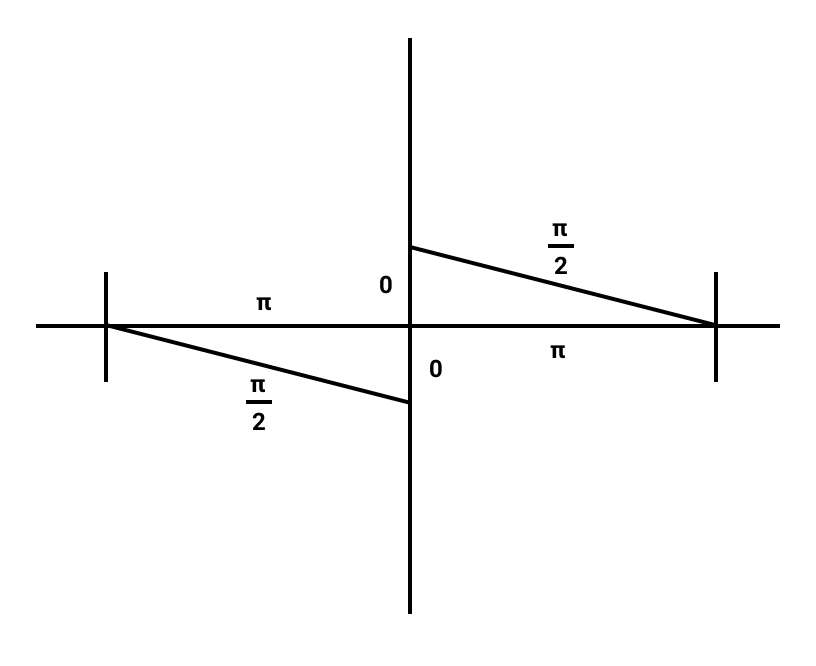
\includegraphics[width=5cm]{more_pictures/horizontal_bowtie.png}
\end{figure}


Furthermore, we can obtain an angle-splitting of $\sT_T(L)$
(and similarly $\sT_B(L)$) by modifying the angle-splitting
for $\sT_T(K)$.

Hmm



\end{proof}


\begin{proof}
By \cite[Theorem 7.5]{CKP2},
$\toruscomp{K}$ can be decomposed
into two torihedra whose graphs are the projection graph of $K$,
which we denote by $\Gamma$.
By assigning angles $\pi/2$ to each edge of the torihedra graphs,
we can invoke \cite[Theorem 3]{BandS} to give us a circle pattern
on the projection graph.

By \prpref{p:tori_decomp}, $\toruscomp{L}$ can be
obtained by gluing two torihedra with graph $\Gamma_T(L)$ and $\Gamma_B(L)$.
Recall that $\Gamma_T(L)$ is obtained from $\Gamma$ by some slight
modifications, specifically by replacing augmented vertices with bow-ties.
We assign angles to edges of the bow-ties as in
\figref{f:bowtie_angles},
and leave untouched edges with the same assignment of $\pi/2$;
we do the same for $\Gamma_B(L)$.

%\begin{figure}
%\label{f:bowtie_angles}
%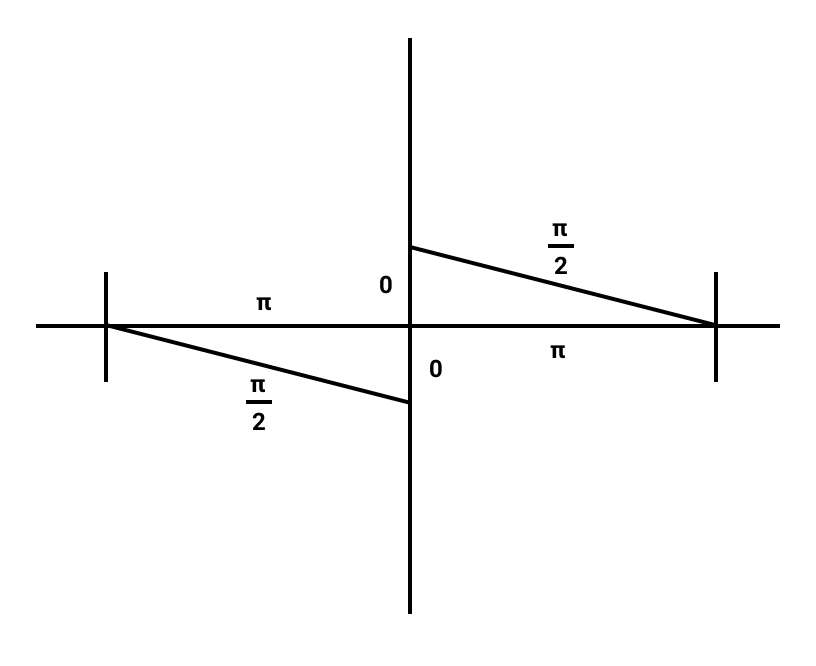
\includegraphics[width=5cm]{more_pictures/horizontal_bowtie.png}
%\end{figure}


(Hmmm... might be misleading, I think $\Psi$ should be a cellular map
$\Gamma_T(L) \to \Gamma_T(K)$, but the latter happens to be
same as $\Gamma$, so that's why it's confusing!)
We can think of a bow-tie in $\Gamma_T(L)$ as ``thickened edges" in the
following sense: consider the bow-tie at a crossing $v$,
and let the edges $e,e'$ of $\Gamma$ at $v$
be associated to the over-strand of $K$.
There is a cellular map from each triangle of the bow-tie
on to $e, e'$ that identifies the $\pi/2$- and 0-labelled edges,
and collapses the $\pi$-labelled edges onto $v$
(TODO see same figure).
It is not hard to see that this map extends to a cellular map
$\Psi: \Gamma_T(L) \to \Gamma$,
and in fact extends to the faces as well.
A similar story applies to $\Gamma_B$.


Now we construct an extended circle pattern for $\Gamma_T(L)$.
We will give a more precise description,
but let us first give the picture.
Under $\Psi$,
each face $f$ of $\Gamma_T(L)$ that is not in a bow-tie
is identified with a face $\bar{f}$ of $\Gamma$,
so we assign the circle of $\bar{f}$ to $f$;
each triangle face $f$ in a bow-tie is collapsed to an edge,
and we assign to $f$ the circle circumscribing the
face of $\Gamma$ that meets $f$ along the 0-labelled edge.
This is a ``degenerate" circle pattern that can be thought of as
the limit of some (singular) circle patterns.


Let us make this more precise,
describing an extended circle pattern $c$
on $\Gamma_T(L)$.
Let the circle pattern for $\Gamma$ be given by
$\bar{c} = ((r_f),(\vphi_{\vec{e}}))$,
where recall $r_f$ is the radius of the circle $C_f$
circumscribing $f$ and $\vphi_{\vec{e}}$
is half the angle subtended by the edge $e$
at the center of $C_f$.
For non-bow-tie faces $f$ of $\Gamma_T(L)$,
$\Psi$ identifies $f$ with the face $\bar{f}$ of $\Gamma$.
We set $r_f(c) = r_{\bar{f}}(\bar{c})$.
For $\vphi$ of its edges,
if $\vec{e} \in \del f$ is labelled $\pi$,
we set $\vphi_{\vec{e}} = 0$;
otherwise, $\Psi$ identifies $\vec{e}$
with the edge $\vec{e}'$ in $\Gamma$,
then we set $\vphi_{\vec{e}}(c) = \vphi_{\vec{e}'}(\bar{c})$.


For a triangular face $f$ of a bow tie,
let $\vec{e}_0, \vec{e}_{\pi/2}, \vec{e}_{\pi}$
be the edges of $f$ labelled $0,\pi/2, \pi$ respectively.
We set $r_f(c) = r_{f'}(c)$,
where $f'$ is the face adjacent to $f$ across $e_0$.
Then we set
$\vphi_{\vec{e}_{\pi/2}} = \vphi_{\cev{e}_0} = \pi - \vphi_{\vec{e}_0}$
and $\vphi_{\vec{e}_{\pi}} = 0$.


It can be easily checked that $c$ satisfies the conditions of
\prpref{p:nghd_lift}.
We would like to apply \lemref{l:circpattern_polyhedra}
to obtain a polyhedral decomposition of the torihedra,
but there are edges with $\vphi_{\vec{e}}$
(specifically, those with $\theta_e = \pi$).
%We want a deformation of $\theta_{\bullet}$ of $c$
%that remains vertex non-singular,
%and gives us an honest ?? circle pattern.
Hence, we want to find a vector $a = \sum a^e \ddd{\theta_e}$
in the tangent space of $\Theta(c)$
that maintains vertex non-singularity,
i.e.  such that $\sum_{e \ni v} a^e = 0$ for all vertices $v$,
and for edges $e$ with $\theta_e = \pi$,
we have $a^e < 0$.
By \prpref{p:nghd_lift}, there exists $\veps > 0$
such that the path $\gamma(t) = \Theta(c) + t \cdot a$, $t\in [0,\veps]$,
in $\TTT$ can be lifted to a path $\tilde{\gamma}$ in $\CCC$.


To find such $a$, we need to modify $\Gamma_T(L)$ by
cutting faces along new edges.
Consider a face $f$ that is not in a bow-tie.
Suppose the corresponding face $\bar{f}$ of $\Gamma$
had vertices $v_1,\ldots,v_n$ in counter-clockwise order.
Suppose it is the case that if a vertex $v_i$ is left-augmented,
then the augmentation circle intersects $\bar{f}$
(everything is similar if it is right-augmented circles that intersect
$\bar{f}$).
Vertex $v_i$ corresponds to one edge $e_i$ of $\Gamma_T(L)$
if $v_i$ is not augmented or right-augmented,
and corresponds to two edges $e_{i,0}, e_{i,\pi}$
of $\Gamma_T(L)$ if $v_i$ is left-augmented
($e_{i,0}, e_{i,\pi}$ are edges of a single bow-tie,
and $e_{i,0}$ has $\theta_{e_{i,0}} = 0$
and $e_{i,\pi}$ has $\theta_{e_{i,\pi}} = \pi$).


Suppose, after cyclically reindexing, $v_1,\ldots,v_k$
is a maximally contiguous subsequence of left-augmented vertices
of $G(K)$ around the face $\bar{f}$;
the edges around $f$ would start
$e_{1,0}, e_{1,\pi}, e_{2,0}, e_{2,\pi}, \ldots$.
We add new edges across $f$ as follows.

First suppose $k=n$; then we do nothing.

Next suppose there is only one such maximal contiguous subsequence.
If $k = 1$, we add an edge that goes across
$e_{1,0},e_{1,\pi},e_2$
(in the sense that the new edge separates the edges of $f$ into two sets
one of them being those three edges;
since $n\geq 3$, this edge is new).
If $k = 2$, we add edge across $e_{1,0},e_{1,\pi}$
and another edge across $e_{2,0},e_{2,\pi}$
(these two edges do not form a bigon because we've ruled out $k=n$).
If $k \geq 3$,
we add an edge across $e_{1,0},e_{1,\pi},e_{2,0}$
and another edge across $e_{2,\pi},e_{3,0},\ldots,e_{k,\pi}$
(again these two edges do not form a bigon).

Finally, if there are multiple such maximal contiguous subsequences,
we just add edges as above for each contiguous subsequence.
The only caveat is that if the procedure calls to add a new edge
that would form a bigon with the existing edges,
we just don't add it.

See \figref{f:adding_edges}


\begin{figure}
\label{f:adding_edges}
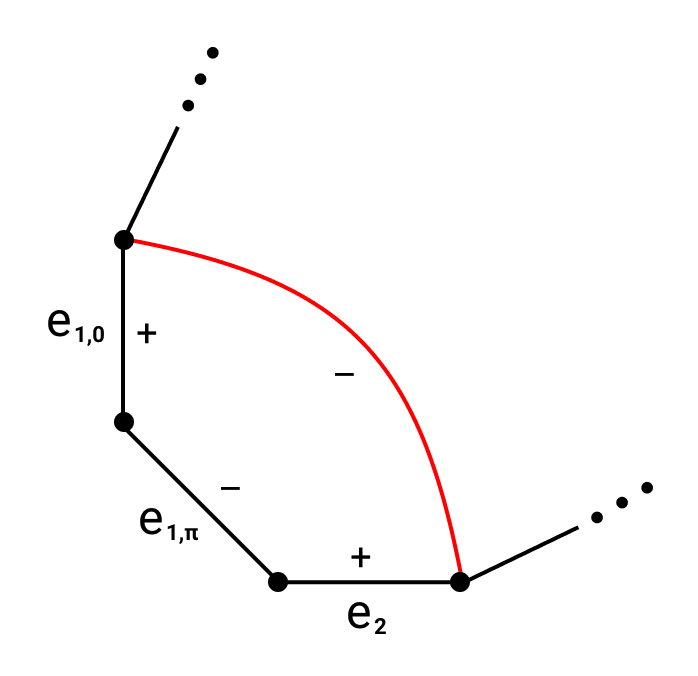
\includegraphics[width=5cm]{more_pictures/one_edge.png}
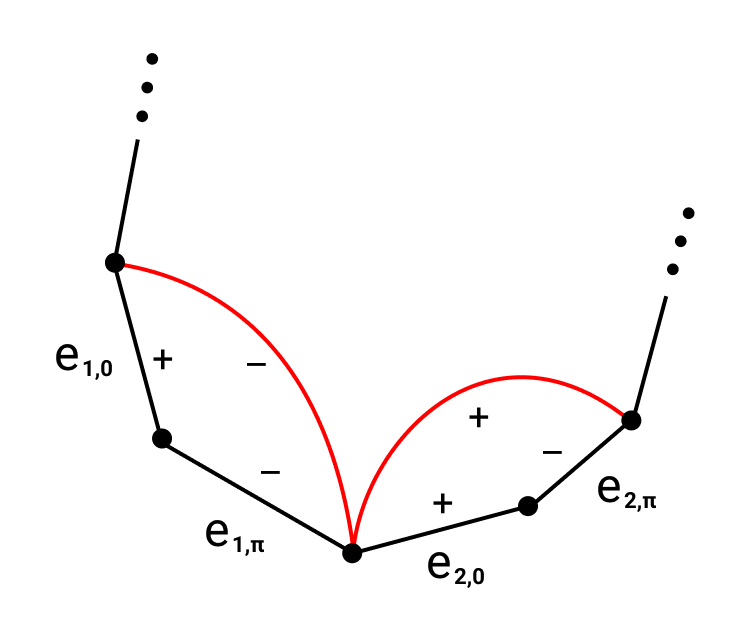
\includegraphics[width=5cm]{more_pictures/two_edge.png}
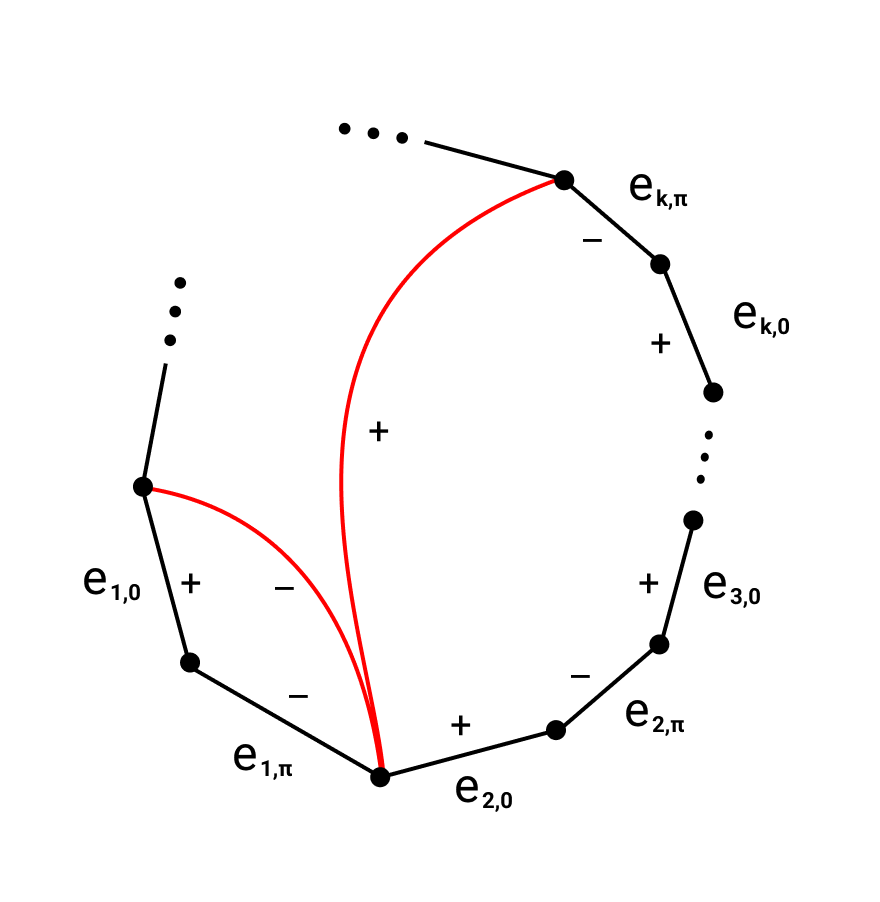
\includegraphics[width=5cm]{more_pictures/two_edge_many.png}
\end{figure}

TODO CONTINUE HERE do the $+$ and $-$ on the edges.




Our torihedral decomposition has graph and on augmentation we will give 0 and pi angles. Next we add another edge and give blah angle (we have three cases)
do three cases with pictures

part 3: Use proposition to get circle pattern to get polyhedral decomposition of the link 

part 4: get triangulation.  

\end{proof}



%%%%%%%%%%%%%%%%%%%%%%%%%%%%%%%%%%%%%%%%%%%%%%%%%%%%%%%%%%%
\section{From Extended Circle Patterns to polyhedra}

In this section, we describe how to obtain a
decomposition of a torihedron
into hyperbolic ideal pyramids
from a non-singular extended circle pattern.

\begin{lemma}
\label{l:circpattern_polyhedra}
Suppose we have the graph of a torihedron.
Given a non-singular extended circle pattern $c \in \CCC$ on the graph,
such that all $\vphi_{\vec{e}} \in (0,\pi)$,
there exists a decomposition of the torihedron
into base-angled ideal pyramids (TODO make sure it's been defined) such that
	\begin{itemize}
		\item each interior edge of the torihedron has dihedral angles sum to $2\pi$;
		\item each boundary edge $e$ of the torihedron has dihedral angles sum to
			$\pi - \theta_e$.
	\end{itemize}
\end{lemma}

\begin{proof}
For each directed edge $\vec{e} \in \vec{E}$,
construct the isosceles triangle $T_{\vec{e}}$
with equal sides of length $r_{f_{\vec{e}}}$ and
angle $2\tilde{\vphi}_{\vec{e}}$ subtended between them,
where $\tilde{\vphi}_{\vec{e}} = \vphi_{\vec{e}}$
if $\vphi_{\vec{e}}$ if it is acute,
and = $\pi - \vphi_{\vec{e}}$ otherwise.

\begin{figure}
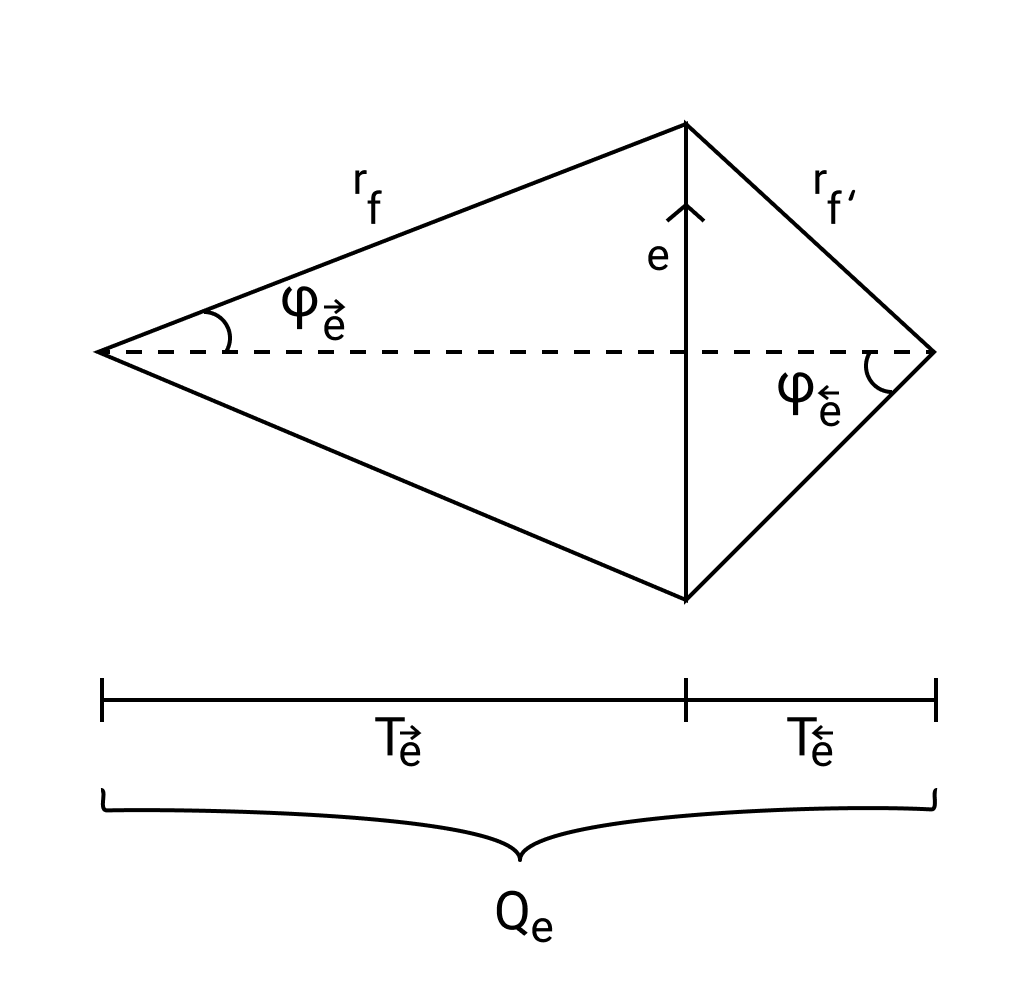
\includegraphics[width=8cm]{more_pictures/kite.png}
\end{figure}
\begin{figure}
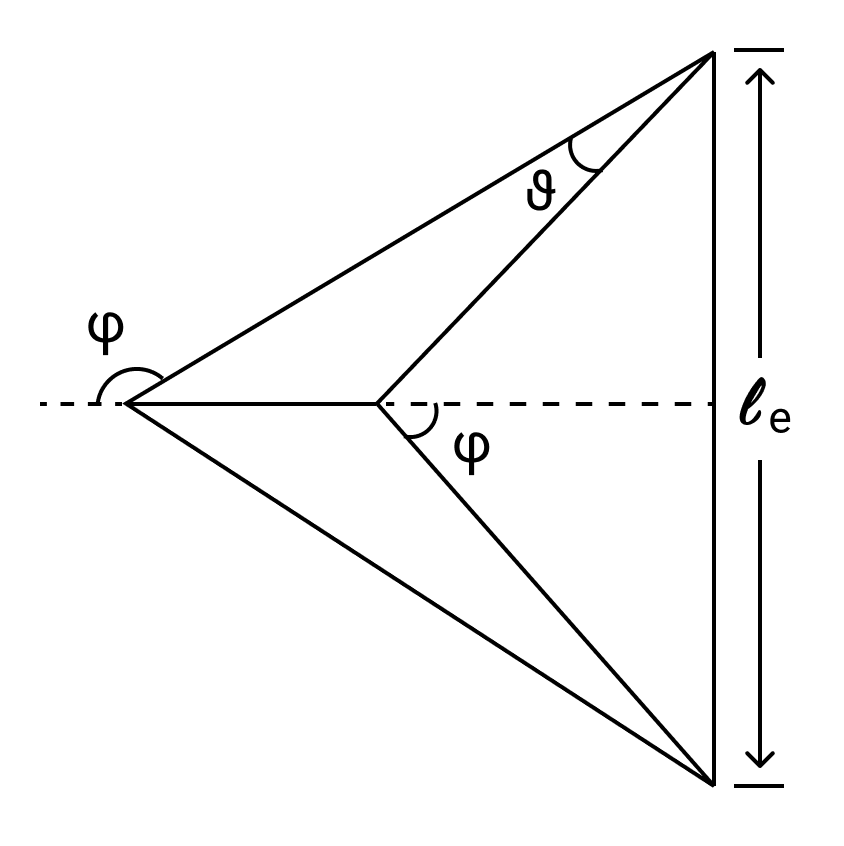
\includegraphics[width=5cm]{more_pictures/positive_angle.png}
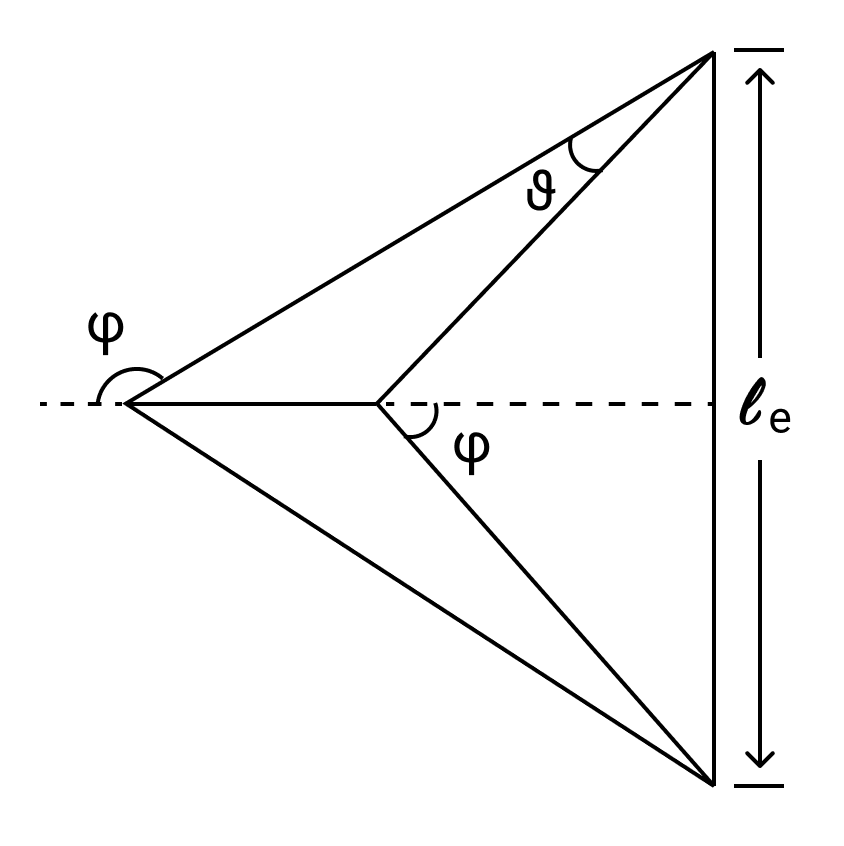
\includegraphics[width=5cm]{more_pictures/negative_angle.png}
\end{figure}


Let $f \in F$ be a face.
We construct a Euclidean polygon $\Pol_f$ as follows.
If $\vphi_{\vec{e}} \leq \pi/2$ for all $\vec{e} \in \del f$,
i.e. if $f$ is convex, then 
the $T_{\vec{e}}$ for $\vec{e}\in \del f$
fit together into $\Pol_f$.
If not, suppose $\vphi_{\vec{e}} > \pi/2$
for $\vec{e} = \vec{e_1}$, 
and $\leq \pi/2$ for $\vec{e} = \vec{e_2},\ldots \vec{e_k} \in \del f$.
Then put $T_{\vec{e_2}},\ldots,T_{\vec{e_k}}$ together as above,
creating a $(k+1)$-gon,
then subtract $T_{\vec{e_1}}$ from it to form $\Pol_f$.

Thus, to each face, we associate the Euclidean polygon $\Pol_f$.
If $v$ is the vertex of $\Pol_f$ between $e_i$ and $e_{i+1}$,
then the angle at $v$ is
$\pi - \vphi_{\vec{e_i}} - \vphi_{\vec{e_{i+1}}}$.
Then the non-vertex-singularity of $c$ guarantees that
the sum of angles at $v$ of $\Pol_f$, for faces $f$ containing $v$,
is $2\pi$.
%; in other words, $\Pol_f$ glue along edges


View the Euclidean plane as the boundary of the upper-half space.
Then $\Pol_f$ supports an ideal hyperbolic pyramid $P_f$.

Clearly, these $P_f$'s, as abstract ideal tetrahedra,
glue together into the torihedron (TODO rephrase).
%The hyperbolic structure on $P_f$
%in particular provide dihedral angles to each edge of $P_f$
%which clearly satisfies the conditions of making $P_f$
%a base-angled ideal pyramid.
We need to check that the angles around each edge of
the torihedron have the appropriate angles.


Consider an interior edge $e$ of the pyramidal decomposition
of the torihedron.
It corresponds to a vertex $v$ of the graph.
Note that the dihedral angle of the vertical edge
at $v$ of $P_f$ is simply the angle at $v$ of $\Pol_f$;
these sum to $2\pi$ over $f \ni v$.


For a boundary edge $e$, the dihedral angles at $e$ of the $P_f$'s
containing it are $\vphi_{\vec{e}}$ and $\vphi_{\cev{e}}$,
which sum to $\theta_e$ by definition.

\end{proof}


\bibliographystyle{plain}
\bibliography{references-ak}


TODO consistent torus symbol, consistent thickened torus symbols

\end{document}
